\documentclass[a4paper,11pt]{article}

\usepackage[utf8]{inputenc}
\usepackage[T1]{fontenc}
\usepackage{lmodern}
\usepackage[brazilian]{babel}
\usepackage[a4paper,margin=1.65cm,top=1.9cm,bottom=1.9cm]{geometry}

\usepackage{amsmath}
\usepackage{amssymb}
\linespread{1.05}
\usepackage{graphicx}
\usepackage{booktabs}
\usepackage{tabularx}
\usepackage{array}
\usepackage{caption}
\usepackage{enumitem}
\usepackage{xcolor}
\usepackage{listings}
\usepackage{url}
\usepackage[
  unicode=true,
  colorlinks=true,
  linkcolor=blue!35!black,
  urlcolor=blue!35!black,
  citecolor=blue!35!black,
  pdftitle={Relatorio Final do Projeto - Aprendizagem de Maquina (IN1102)},
  pdfauthor={Douglas Araujo Silva, Felipe Araujo de Lima, Leticia De Albuquerque S. Leitao}
]{hyperref}

\captionsetup{font=small,labelfont=bf,hypcap=false}
\setlength{\parindent}{0pt}
\setlength{\parskip}{0.45em}
\setlength{\emergencystretch}{2.5em}
\setcounter{tocdepth}{3}
\setcounter{secnumdepth}{4}

\newcolumntype{L}{>{\raggedright\arraybackslash}X}
\newcolumntype{C}{>{\centering\arraybackslash}X}
\newcolumntype{P}[1]{>{\raggedright\arraybackslash}p{#1}}
\newcolumntype{Q}[1]{>{\centering\arraybackslash}p{#1}}
\newcolumntype{R}[1]{>{\raggedleft\arraybackslash}p{#1}}

\definecolor{codebg}{HTML}{F7F8FA}
\definecolor{codeframe}{HTML}{D0D7DE}
\definecolor{notebg}{HTML}{F4F6F9}

\lstset{
  basicstyle=\ttfamily\footnotesize,
  backgroundcolor=\color{codebg},
  frame=single,
  rulecolor=\color{codeframe},
  breaklines=true,
  breakatwhitespace=false,
  columns=fullflexible,
  keepspaces=true,
  xleftmargin=0.6em,
  xrightmargin=0.6em,
  aboveskip=0.7em,
  belowskip=0.7em,
  literate=
    {á}{{\'a}}1 {à}{{\`a}}1 {â}{{\^a}}1 {ã}{{\~a}}1
    {é}{{\'e}}1 {ê}{{\^e}}1 {í}{{\'i}}1
    {ó}{{\'o}}1 {ô}{{\^o}}1 {õ}{{\~o}}1 {ú}{{\'u}}1
    {ç}{{\c{c}}}1
    {Á}{{\'A}}1 {À}{{\`A}}1 {Â}{{\^A}}1 {Ã}{{\~A}}1
    {É}{{\'E}}1 {Ê}{{\^E}}1 {Í}{{\'I}}1
    {Ó}{{\'O}}1 {Ô}{{\^O}}1 {Õ}{{\~O}}1 {Ú}{{\'U}}1
    {Ç}{{\c{C}}}1
}

\renewcommand{\contentsname}{Sumário}

\begin{document}

\begin{center}
  {\LARGE\bfseries Relatório Final do Projeto\par}
  \vspace{0.45em}
  {\large Disciplina de Aprendizagem de Máquina (IN1102, pós-graduação)\par}
  \vspace{0.3em}
  {\normalsize Grupo: Douglas Araújo Silva, Felipe Araújo de Lima, Letícia De Albuquerque S. Leitão\par}
  \vspace{0.2em}
  {\normalsize\bfseries 2026.2\par}
\end{center}
\noindent\rule{\linewidth}{0.7pt}\par
\vspace{-1.2em}
\phantomsection
\section*{Resumo}
\addcontentsline{toc}{section}{Resumo}
\label{sec:resumo}


Este relatório consolida o desenvolvimento metodológico, os experimentos computacionais, a análise estatística e os mecanismos de reprodutibilidade do projeto da disciplina \textbf{Aprendizagem de Máquina (IN1102 --- CIn/UFPE, 2026.2)} aplicado à base de dados \textbf{Spambase} ($4.601$ e-mails, $57$ atributos numéricos contínuos e rótulo binário original \texttt{non-spam}/\texttt{spam}).

Na \textbf{Questão 1 (aprendizagem não supervisionada)}, implementou-se e validou-se o algoritmo \textbf{Double K-means} (\textit{co-clustering} simultâneo de instâncias e atributos) sobre uma grade de $9$ pares $(K, H)$ com $K \in \{2, 3, 4\}$ e $H \in \{1, \ldots, K\}$, executando $100$ reinicializações válidas por par ($900$ execuções válidas por estratégia) com sementes determinísticas. Em cada representação, a escolha dos hiperparâmetros seguiu o critério em dois estágios: menor função objetivo $W$ entre os \textit{restarts} e, em seguida, escolha de $(K^*, H^*) = \arg\max_{(K,H)} \text{Sil}((K,H))$. Uma investigação sistemática de sensibilidade ao pré-processamento comparou $7$ tratamentos distintos ($6.300$ execuções válidas ao todo), demonstrando que a padronização clássica z-score (\texttt{StandardScaler} puro, linha de base \texttt{revisada}) sofre do chamado \textbf{``Paradoxo da Silhueta''}: ao isolar um microcluster de apenas $34$ mensagens legítimas ($0,74\%$) com vocabulário técnico específico frente às demais $4.567$ ($99,26\%$), atinge Silhueta Euclidiana de $0,6596$, mas concordância externa nula com as classes originais ($\text{ARI} = -0,00495$). Para a Questão 2, adotou-se a representação \texttt{log\_\allowbreak minmax} ($\log(1+x)$ seguida de \texttt{MinMaxScaler}), tanto pelo tratamento das caudas pesadas sem descartar variáveis quanto pela concordância externa observada via ARI após o agrupamento. O ARI informou a decisão \textbf{entre representações}, mas não participou do agrupamento nem da escolha de $(K,H)$ \textbf{dentro de cada representação}. Nessa representação, obteve-se $(K^*, H^*) = (3, 3)$ ($W = 2.906,2307$, Silhueta $= 0,129219$, $\text{ARI} = +0,391111$, grupos de $2.619$, $265$ e $1.717$ instâncias). O arquivo exportado para a Questão 2 (\texttt{spambase\_\allowbreak q2.csv}, verificado por hash SHA-256) preservou integralmente os $57$ atributos em \textbf{escala bruta original}.

Na \textbf{Questão 2 (aprendizagem supervisionada)}, avaliaram-se cinco classificadores --- \textbf{Bayesiano Gaussiano Multivariado}, \textbf{Bayes k-NN}, \textbf{Bayes Parzen} (kernel gaussiano multivariado produto), \textbf{Regressão Logística} e \textbf{Voto Majoritário} --- nas duas versões do alvo (\texttt{y\_\allowbreak original} com $2$ classes e \texttt{y\_\allowbreak double\_\allowbreak kmeans} com $3$ clusters). O protocolo empregou validação cruzada estratificada \textbf{30 $\times$ 10-folds} ($3.000$ avaliações externas; $1.380.300$ predições auditadas), com \textbf{CV 5-folds interna} restrita aos $9$ folds de treino externo para seleção de hiperparâmetros e ajuste de \texttt{log1p + MinMaxScaler} estritamente dentro de cada partição de treino, evitando \textit{data leakage}. Em \texttt{y\_\allowbreak original}, \textbf{Voto Majoritário} ($\text{F1 macro} = 0,9397$, taxa de erro $= 5,71\%$) e \textbf{Bayes Parzen} ($\text{F1 macro} = 0,9394$, taxa de erro $= 5,75\%$) lideraram, sem diferença detectada entre si pelo pós-teste exploratório de Nemenyi ($p = 0,9883$). Em \texttt{y\_\allowbreak double\_\allowbreak kmeans}, a \textbf{Regressão Logística} obteve o melhor desempenho ($\text{F1 macro} = 0,9827$, erro $= 0,95\%$), superando Voto Majoritário ($0,9347$), Parzen ($0,9224$), k-NN ($0,9114$) e Gaussiano ($0,7976$), com $p = 0,1024$ entre Logística e Voto no Nemenyi exploratório ($\text{CD} = 1,1136$). Um estudo complementar ($1 \times 10$-folds, $300$ avaliações) corroborou exploratoriamente a escolha de \texttt{log1p + MinMaxScaler} sobre dados brutos e \texttt{MinMaxScaler} isolado, e curvas de aprendizagem estratificadas ($5\%$ a $95\%$ em passo de $5\%$) caracterizaram o comportamento treino-teste sob diferentes tamanhos amostrais. Ao final, toda a suíte unificada do repositório alcança \textbf{$71$ testes automatizados aprovados} ($4$ testes e $14$ subtestes na Questão 1; $67$ testes e $29$ subtestes na Questão 2).


\tableofcontents
\newpage


\section{Introdução}\label{sec:1-introducao}


A filtragem automática de mensagens indesejadas (\textit{spam}) e a descoberta de estruturas latentes em coleções textuais representam problemas clássicos de Aprendizagem de Máquina que exigem cuidado experimental tanto na representação numérica dos atributos quanto na separação rigorosa entre conjuntos de treinamento, validação e teste.

Este relatório documenta o cumprimento integral das duas frentes especificadas no enunciado oficial da disciplina (Projeto-AM-2026-2.pdf), utilizando a base \textbf{Spambase} em um fluxo experimental encadeado, auditado e reproduzível.

\subsection{Objetivos do Projeto}\label{sec:1-1-objetivos-do-projeto}


\begin{enumerate}[leftmargin=1.5em, itemsep=0.25em, topsep=0.25em]
  \item \textbf{Questão 1 (Co-clustering não supervisionado):}
\begin{itemize}[leftmargin=1.5em, itemsep=0.25em, topsep=0.25em]
  \item Aplicar o algoritmo \textbf{Double K-means} à matriz de atributos do Spambase (sem qualquer acesso à classe original), executando $100$ reinicializações válidas para cada par $(K, H)$ com $K \in \{2, 3, 4\}$ e $H \in \{1, \ldots, K\}$.
  \item Selecionar, em cada par $(K, H)$, a solução de menor função objetivo $W$, computar sua Silhueta Euclidiana média, escolher $(K^*, H^*) = \arg\max_{(K,H)} \text{Sil}((K,H))$ e avaliar \textit{a posteriori} a concordância com as classes originais via \textit{Adjusted Rand Index} (ARI).
  \item Reportar a matriz de protótipos dos blocos ($G$), a matriz de confusão/contingência frente à partição \textit{a priori}, a evolução de $W$ ao longo das iterações e investigar criticamente a sensibilidade do algoritmo ao pré-processamento.
\end{itemize}
  \item \textbf{Questão 2 (Classificação supervisionada e comparação estatística):}
\begin{itemize}[leftmargin=1.5em, itemsep=0.25em, topsep=0.25em]
  \item Construir duas tarefas supervisionadas distintas sobre os mesmos $57$ preditores em escala bruta: \texttt{y\_\allowbreak original} ($2$ classes originais) e \texttt{y\_\allowbreak double\_\allowbreak kmeans} ($K^*$ clusters descobertos na Questão 1).
  \item Avaliar e comparar cinco classificadores --- \textbf{Bayesiano Gaussiano Multivariado}, \textbf{Bayes k-vizinhos (k-NN)}, \textbf{Bayes baseado em janela de Parzen} (kernel gaussiano multivariado produto), \textbf{Regressão Logística} e \textbf{Voto Majoritário} --- sob validação cruzada estratificada \textbf{30 $\times$ 10-folds}, com ajuste de hiperparâmetros via \textbf{5-folds internos} restritos aos $9$ folds de treino externo e retreino nos $9$ folds.
  \item Obter estimativas pontuais e intervalos de confiança para Taxa de erro, Precisão, Cobertura e F-measure; comparar os modelos pelo teste de \textbf{Friedman} e pós-teste de \textbf{Nemenyi} em todas as métricas; e construir e comentar curvas de aprendizagem de F-measure em treinamento e teste de $5\%$ a $95\%$ (passo de $5\%$).
\end{itemize}
\end{enumerate}
\subsection{\texorpdfstring{Descrição Sucinta dos Dados (\textit{Spambase})}{Descrição Sucinta dos Dados (Spambase)}}\label{sec:1-2-descricao-sucinta-dos-dados-spambase}


O conjunto de dados \textbf{Spambase}, originalmente doado pelos laboratórios \textit{Hewlett-Packard} (HP Labs) ao \textit{UCI Machine Learning Repository} (\texttt{https:/\allowbreak /\allowbreak archive.ics.uci.edu/\allowbreak dataset/\allowbreak 94/\allowbreak spambase}), é armazenado no repositório em \texttt{data/\allowbreak raw/\allowbreak spambase.data} e documentado em \texttt{data/\allowbreak raw/\allowbreak spambase.names}.

\begin{itemize}[leftmargin=1.5em, itemsep=0.25em, topsep=0.25em]
  \item \textbf{Dimensões:} $N = 4.601$ instâncias (e-mails), $P = 57$ atributos numéricos contínuos não negativos, sem valores ausentes ou infinitos.
  \item \textbf{Variável alvo original (\texttt{y\_\allowbreak original}):}
\begin{itemize}[leftmargin=1.5em, itemsep=0.25em, topsep=0.25em]
  \item Classe \texttt{0} (\textit{non-spam} / legítimo): \textbf{$2.788$ instâncias} ($60,60\%$);
  \item Classe \texttt{1} (\textit{spam} / não solicitado): \textbf{$1.813$ instâncias} ($39,40\%$).
\end{itemize}
  \item \textbf{Estrutura dos 57 atributos preditores:}
\begin{enumerate}[leftmargin=1.5em, itemsep=0.25em, topsep=0.25em]
  \item \textbf{Frequências de palavras (\texttt{0} a \texttt{47}, $48$ atributos \texttt{word\_\allowbreak freq\_\allowbreak WORD}):} percentual em $[0, 100]$ das palavras do e-mail que coincidem com termos como \texttt{make}, \texttt{address}, \texttt{free}, \texttt{money}, \texttt{remove}, \texttt{hp}, \texttt{hpl}, \texttt{george}, \texttt{415}, \texttt{857}, \texttt{telnet}, \texttt{technology}, entre outros.
  \item \textbf{Frequências de caracteres (\texttt{48} a \texttt{53}, $6$ atributos \texttt{char\_\allowbreak freq\_\allowbreak CHAR}):} percentual em $[0, 100]$ das ocorrências dos caracteres \texttt{;}, \texttt{(\allowbreak }, \texttt{[}, \texttt{!}, \texttt{\$}, \texttt{\#}.
  \item \textbf{Sequências de letras maiúsculas (\texttt{54} a \texttt{56}, $3$ atributos):}
\begin{itemize}[leftmargin=1.5em, itemsep=0.25em, topsep=0.25em]
  \item \texttt{capital\_\allowbreak run\_\allowbreak length\_\allowbreak average}: comprimento médio das sequências ininterruptas de maiúsculas (valor real contínuo $\ge 1$);
  \item \texttt{capital\_\allowbreak run\_\allowbreak length\_\allowbreak longest}: comprimento máximo de uma sequência ininterrupta de maiúsculas (inteiro contínuo $\ge 1$);
  \item \texttt{capital\_\allowbreak run\_\allowbreak length\_\allowbreak total}: soma total de letras maiúsculas no e-mail (inteiro contínuo $\ge 1$).
\end{itemize}
\end{enumerate}
\end{itemize}
Do ponto de vista estatístico, a base apresenta três propriedades críticas para métodos baseados em distância e covariância:
\begin{enumerate}[leftmargin=1.5em, itemsep=0.25em, topsep=0.25em]
  \item \textbf{Alta esparsidade:} nos atributos de frequência de palavras e caracteres, mais de $80\%$ das entradas são iguais a zero;
  \item \textbf{Assimetria positiva acentuada e caudas pesadas:} termos raros permanecem zerados na maioria dos e-mails, mas atingem picos elevados em subconjuntos restritos (por exemplo, \texttt{word\_\allowbreak freq\_\allowbreak 415} atinge $4,76\%$, correspondendo a $z \approx +14,30$ sob padronização z-score global);
  \item \textbf{Discrepância severa de escalas:} enquanto frequências percentuais variam tipicamente de $0$ a algumas unidades ou dezenas, \texttt{capital\_\allowbreak run\_\allowbreak length\_\allowbreak total} possui média $283$, desvio-padrão $606$ e máximo $15.841$, e \texttt{capital\_\allowbreak run\_\allowbreak length\_\allowbreak longest} atinge escore padronizado $z \approx +50,99$ sem compressão logarítmica.
\end{enumerate}

\section{Etapas e Andamento do Projeto}\label{sec:2-etapas-e-andamento-do-projeto}


\subsection{Questão 1 --- Agrupamento Co-clustering via Double K-means}\label{sec:2-1-questao-1-agrupamento-co-clustering-via-double-k-means}


\subsubsection{Formulação Matemática e Otimização}\label{sec:2-1-1-formulacao-matematica-e-otimizacao}


Implementado em \texttt{questao1/\allowbreak src/\allowbreak double\_\allowbreak kmeans.py}, o algoritmo \textbf{Double K-means} particiona simultaneamente as $N$ linhas (e-mails) em $K$ grupos $U \in \{0,1\}^{N \times K}$ ($\sum_{k=1}^K u_{ik} = 1$) e as $P$ colunas (atributos) em $H$ grupos $V \in \{0,1\}^{P \times H}$ ($\sum_{h=1}^H v_{jh} = 1$), resumindo cada co-cluster pela matriz de protótipos de blocos $G = [g_{kh}] \in \mathbb{R}^{K \times H}$. A função objetivo minimizada é a inércia quadrática intrabloco:

\[
W(G, U, V) = \sum_{k=1}^{K} \sum_{h=1}^{H} \sum_{i=1}^{N} \sum_{j=1}^{P} u_{ik} v_{jh} (x_{ij} - g_{kh})^2
\]

Partindo de partições aleatórias iniciais \textit{hard} que garantem ao menos um objeto em cada cluster de linhas e ao menos uma variável em cada cluster de colunas (\texttt{\_\allowbreak initial\_\allowbreak partition}), a otimização alterna três passos determinísticos a cada iteração:

\begin{enumerate}[leftmargin=1.5em, itemsep=0.25em, topsep=0.25em]
  \item \textbf{Atualização da matriz de protótipos $G$ ($U, V$ fixos):}
\[
g_{kh} = \frac{1}{|C_k| \cdot |D_h|} \sum_{i \in C_k} \sum_{j \in D_h} x_{ij}
\]
onde $C_k = \{i \mid u_{ik} = 1\}$ e $D_h = \{j \mid v_{jh} = 1\}$.
  \item \textbf{Atualização da partição de objetos $U$ ($G, V$ fixos):} atribui cada objeto $i$ ao grupo $k^*$ que minimiza $\sum_{h=1}^H \sum_{j \in D_h} (x_{ij} - g_{kh})^2$.
  \item \textbf{Atualização da partição de variáveis $V$ ($G, U$ fixos):} atribui cada variável $j$ ao grupo $h^*$ que minimiza $\sum_{k=1}^K \sum_{i \in C_k} (x_{ij} - g_{kh})^2$.
\end{enumerate}
\textbf{Critério de parada, monotonicidade e descarte de degenerescências:}
\begin{itemize}[leftmargin=1.5em, itemsep=0.25em, topsep=0.25em]
  \item O algoritmo converge quando \textbf{não ocorrem transferências} em nenhuma das duas partições entre iterações sucessivas (\texttt{object\_\allowbreak labels} e \texttt{variable\_\allowbreak labels} idênticos aos da iteração anterior), ou ao atingir o teto \texttt{max\_\allowbreak iter =\allowbreak  200} iterações.
  \item Verifica-se a cada passo se $W \le W_{\text{anterior}} + \text{monotonic\_tol}$ com \texttt{monotonic\_\allowbreak tol =\allowbreak  1e-7}.
  \item Se em qualquer etapa algum cluster de objetos ou de variáveis ficar vazio ($|C_k| = 0$ ou $|D_h| = 0$), a execução retorna \texttt{None}, é contabilizada em \texttt{invalid\_\allowbreak attempts} e descartada até que se completem exatamente \textbf{$100$ execuções válidas} por par $(K, H)$ (com limite de segurança \texttt{max\_\allowbreak attempts =\allowbreak  50 * n\_\allowbreak restarts}).
\end{itemize}
\subsubsection{Obtenção dos Hiperparâmetros (K, H) e Seleção em Dois Estágios}\label{sec:2-1-2-obtencao-dos-hiperparametros-k-h-e-selecao-em-dois-estagios}


Conforme o protocolo não supervisionado implementado em \texttt{questao1/\allowbreak src/\allowbreak experimento.py}:

\begin{itemize}[leftmargin=1.5em, itemsep=0.25em, topsep=0.25em]
  \item \textbf{Grade completa ($9$ pares):} $K \in \{2, 3, 4\}$ e $H \in \{1, \ldots, K\}$, isto é, $(2,1),\allowbreak (2,2),\allowbreak (3,1),\allowbreak (3,2),\allowbreak (3,3),\allowbreak (4,1),\allowbreak (4,2),\allowbreak (4,3),\allowbreak (4,4)$.
  \item \textbf{Restarts e sementes determinísticas:} cada par executa $100$ rodadas válidas com sementes regidas por:
\[
\text{seed} = \text{base\_seed} + 10.000 \cdot K + 1.000 \cdot H + \text{attempt}, \qquad \text{base\_seed} = 42
\]
  \item \textbf{Invariante de seleção em cascata (aplicado separadamente a cada representação):}
\begin{enumerate}[leftmargin=1.5em, itemsep=0.25em, topsep=0.25em]
  \item \textit{Estágio 1 (interno ao par):} seleciona-se entre as $100$ execuções válidas \textbf{exclusivamente aquela de menor função objetivo $W$}; nunca se seleciona \textit{restart} pela Silhueta.
  \item \textit{Estágio 2 (entre os 9 pares):} calcula-se a Silhueta Euclidiana média sobre a partição de objetos vencedora por $W$, definindo $(K^*, H^*) = \arg\max_{(K,H)} \text{Sil}((K,H))$.
  \item \textit{Avaliação externa a posteriori:} apenas após a fixação de $(K^*, H^*)$ compara-se a partição descoberta com \texttt{y\_\allowbreak original} via \textit{Adjusted Rand Index} (ARI). A coluna \texttt{y\_\allowbreak original} não participa das transformações dos atributos, das atualizações de $U$, $V$, $G$ nem da escolha de $(K^*, H^*)$ \textbf{dentro da representação avaliada}. Entretanto, o ARI calculado depois do agrupamento foi considerado na \textbf{decisão entre as sete representações}, etapa adicional informada pelos rótulos conhecidos.
\end{enumerate}
\end{itemize}
\subsubsection{Comparação de Estratégias de Pré-processamento (6.300 Execuções)}\label{sec:2-1-3-comparacao-de-estrategias-de-pre-processamento-6-300-execucoes}


Como o enunciado não fixa uma transformação prévia obrigatória para o Double K-means, conduziu-se uma investigação complementar de sensibilidade ao pré-processamento em \texttt{questao1/\allowbreak src/\allowbreak preprocessamentos.py} comparando a linha de base (\texttt{revisada}, com \texttt{StandardScaler} puro) e seis estratégias alternativas sob exatamente a mesma grade, sementes e critério de seleção ($900$ execuções válidas por estratégia; $6.300$ ao todo).

\textbf{Hipóteses e fundamentação conceitual da escolha das 7 estratégias:} considerando que o Double K-means resume cada bloco $(C_k, D_h)$ por uma única média escalar $g_{kh}$ sob perda quadrática $W$, o conjunto foi delineado como um experimento diagnóstico progressivo para dados não negativos, esparsos ($>80\%$ zeros) e de cauda pesada:
\begin{enumerate}[leftmargin=1.5em, itemsep=0.25em, topsep=0.25em]
  \item \textbf{Linha de base linear (\texttt{revisada} --- \texttt{StandardScaler} puro):} padroniza média zero e variância unitária, mas preserva a assimetria positiva, gerando escores $z$ extremos (até $+50,99$ nas maiúsculas e $+14,30$ em termos raros) que dominam $W$.
  \item \textbf{Duas estratégias diagnósticas de causa (ablação):} \texttt{tratamento\_\allowbreak diferenciado\_\allowbreak runs} (\texttt{log1p} apenas nas $3$ maiúsculas + \texttt{StandardScaler}) testa se o isolamento de \textit{outliers} decorria apenas da escala das maiúsculas frente às frequências percentuais; \texttt{filtragem\_\allowbreak dominio} (remoção de $8$ termos específicos + \texttt{StandardScaler}) testa a sensibilidade ao subconjunto lexical raro associado ao contexto HP Labs, avaliando o custo de descartar atributos originais.
  \item \textbf{Quatro famílias de correção preservando os $57$ atributos:} \texttt{binarizacao} ($x > 0$ nas $54$ frequências + \texttt{log1p} nas $3$ maiúsculas + \texttt{StandardScaler}) suprime o efeito de cauda mantendo apenas presença/ausência; \texttt{clip\_\allowbreak log\_\allowbreak standard} (quantil $99\%$ + \texttt{log1p} + \texttt{StandardScaler}) aplica contenção explícita de extremos (\textit{winsorization}); \texttt{quantile\_\allowbreak uniform} (\texttt{QuantileTransformer} uniforme) realiza mapeamento não paramétrico para $[0,1]$, neutralizando caudas ao custo de alterar distâncias relativas em variáveis esparsas; e \texttt{log\_\allowbreak minmax} ($\log(1+x)$ + \texttt{MinMaxScaler}) comprime monotonicamente as caudas preservando zeros ($0 \mapsto 0$) e confina todas as $57$ variáveis em $[0,1]$, assegurando comensurabilidade dos protótipos $g_{kh}$ sem truncar ou descartar atributos.
\end{enumerate}

\begin{center}
\begin{minipage}{\linewidth}
\centering
\captionof{table}{Comparação sistemática de 7 estratégias de pré-processamento na Questão 1 ($6.300$ execuções válidas).}
\scriptsize
\sloppy
\setlength{\tabcolsep}{2.5pt}
\renewcommand{\arraystretch}{1.18}
\begin{tabularx}{\linewidth}{P{1.90cm} >{\hsize=0.90\hsize}L Q{0.92cm} Q{1.30cm} R{1.34cm} Q{0.82cm} R{1.38cm} Q{1.56cm} >{\hsize=1.10\hsize}L}
\toprule
\textbf{Estratégia} & \textbf{Pré-processamento Aplicado} & \textbf{Par $(K^*, H^*)$} & \textbf{Silhueta Euclidiana} & \textbf{Melhor $W$} & \textbf{Melhor Seed} & \textbf{ARI (vs \texttt{y\_\allowbreak original})} & \textbf{Tamanhos dos Clusters ($N=4.601$)} & \textbf{Diagnóstico Metodológico} \\
\midrule
\textbf{\texttt{revisada}} \textit{(Linha de base)} & \texttt{StandardScaler} puro global ($57$ atributos) & $(2, 2)$ & \textbf{0,659631} & 244.486,70 & 22042 & \textbf{$-$0,004950} & 34 / 4.567 & Isola microcluster de 34 \textit{non-spam} por vocabulário técnico específico; Silhueta artificialmente inflada. \\
\textbf{\texttt{binarizacao}} & Presença binária \texttt{(\allowbreak x > 0)} nas $54$ frequências + \texttt{log1p} nas $3$ maiúsculas + \texttt{StandardScaler} & $(3, 3)$ & 0,210019 & 208.777,15 & 33337 & +0,269498 & 1.344 / 3.025 / 232 & Elimina o microcluster de 34; no par $(2,2)$ atinge ARI $= +0,3553$ (3.228 vs 1.373). \\
\textbf{\texttt{log\_\allowbreak minmax}} \textit{(Oficial Q2)} & $\log(1+x)$ seguida de \texttt{MinMaxScaler} em $[0, 1]^{57}$ & $(3, 3)$ & 0,129219 & 2.906,23 & 33044 & \textbf{+0,391111} & 2.619 / 265 / 1.717 & Comprime caudas pesadas preservando todas as $57$ variáveis; maior ARI entre as vencedoras por Silhueta. \\
\textbf{\texttt{quantile\_\allowbreak uniform}} & \texttt{QuantileTransformer(\allowbreak output\_\allowbreak distribution=\allowbreak 'uniform',\allowbreak  random\_\allowbreak state=\allowbreak 42)} & $(3, 3)$ & 0,190317 & 21.926,53 & 33087 & +0,292525 & 2.787 / 1.240 / 574 & Mapeamento não paramétrico uniforme por quantis; elimina microcluster de 34. \\
\textbf{\texttt{clip\_\allowbreak log\_\allowbreak standard}} & Truncamento no quantil $99\%$ por coluna + \texttt{log1p} + \texttt{StandardScaler} & $(2, 1)$ & 0,172059 & 251.544,66 & 21042 & +0,129196 & 1.372 / 3.229 & Mantém $H=1$; em $(2,2)$ alcançou ARI $= +0,5517$ (Sil $= 0,1085$), mas não venceu o critério de seleção. \\
\textbf{\texttt{filtragem\_\allowbreak dominio}} & Remoção de $8$ termos específicos (\texttt{hp}, \texttt{hpl}, \texttt{george}, \texttt{lab}, \texttt{labs}, \texttt{650}, \texttt{415}, \texttt{857}) + \texttt{StandardScaler} ($49$ variáveis) & $(2, 1)$ & 0,292614 & 220.269,24 & 21042 & +0,136301 & 1.129 / 3.472 & Confirma sensibilidade ao bloco lexical: remove microcluster de 34; em $(2,2)$ obteve ARI $= +0,3607$. \\
\textbf{\texttt{tratamento\_\allowbreak diferenciado\_\allowbreak runs}} & \texttt{StandardScaler} nas $54$ frequências + \texttt{StandardScaler(\allowbreak log1p)} nas $3$ maiúsculas & $(2, 2)$ & 0,653702 & 244.485,00 & 22116 & $-$0,004950 & 4.567 / 34 & Mostra que comprimir apenas maiúsculas não dissolve o microcluster de 34 no par vencedor; em $(3,3)$ ARI $= +0,4632$. \\
\bottomrule
\end{tabularx}
\end{minipage}
\end{center}


\begin{center}
\colorbox{notebg}{\parbox{\dimexpr\linewidth-2\fboxsep\relax}{\small \textbf{Comparabilidade entre representações:} os valores de $W$ e da Silhueta foram calculados em espaços transformados diferentes; seus valores absolutos não devem ser comparados como se compartilhassem a mesma geometria e escala. A seleção por Silhueta ocorreu \textbf{dentro dos nove pares de cada representação}. A decisão posterior por \texttt{log\_\allowbreak minmax} considerou a preservação dos $57$ atributos, o tratamento das caudas e o ARI observado após cada agrupamento. Por utilizar os rótulos conhecidos nessa última decisão, a escolha \textbf{entre representações não foi completamente não supervisionada}; o agrupamento e a seleção de $(K,H)$ em cada representação, sim.}}
\end{center}


\subsubsection{\texorpdfstring{Diagnóstico da Linha de Base (\texttt{revisada}): o Paradoxo da Silhueta}{Diagnóstico da Linha de Base (revisada): o Paradoxo da Silhueta}}\label{sec:2-1-4-diagnostico-da-linha-de-base-revisada-o-paradoxo-da-silhueta}


A auditoria conduzida por \texttt{questao1/\allowbreak src/\allowbreak auditoria.py} sobre a linha de base (\texttt{StandardScaler} puro, $(K^*, H^*) = (2,2)$, \texttt{seed =\allowbreak  22042}, $W = 244.486,6983$, $\text{Sil} = 0,659631$) explica por que uma Silhueta aparentemente alta produziu $\text{ARI} = -0,004950$:

\begin{itemize}[leftmargin=1.5em, itemsep=0.25em, topsep=0.25em]
  \item \textbf{Partição de variáveis ($H^* = 2$):} conforme \texttt{particao\_\allowbreak variaveis.csv}, o grupo de variáveis \texttt{0} concentrou exatamente \textbf{$11$ termos técnicos específicos}: \texttt{word\_\allowbreak freq\_\allowbreak 415}, \texttt{650}, \texttt{85}, \texttt{857}, \texttt{direct}, \texttt{hp}, \texttt{hpl}, \texttt{lab}, \texttt{labs}, \texttt{technology} e \texttt{telnet}. O grupo \texttt{1} agregou as $46$ variáveis restantes.
  \item \textbf{Matriz de protótipos $G$} (\texttt{matriz\_\allowbreak prototipos\_\allowbreak G.csv}):
\end{itemize}
\begin{center}
\begin{minipage}{\linewidth}
\centering
\captionof{table}{Matriz de protótipos $G$ na estratégia linha de base (\texttt{revisada}, $(K^*,H^*)=(2,2)$).}
\small
\setlength{\tabcolsep}{5pt}
\renewcommand{\arraystretch}{1.18}
\begin{tabular}{l c c}
\toprule
\textbf{Grupo de Objetos} & \textbf{Variáveis \texttt{0} (11 termos específicos)} & \textbf{Variáveis \texttt{1} (46 atributos gerais)} \\
\midrule
\textbf{Cluster 0 ($34$ objetos)} & \textbf{+6,861185} & $-$0,144405 \\
\textbf{Cluster 1 ($4.567$ objetos)} & $-$0,051080 & +0,001075 \\
\bottomrule
\end{tabular}
\end{minipage}
\end{center}


\begin{itemize}[leftmargin=1.5em, itemsep=0.25em, topsep=0.25em]
  \item \textbf{Matriz de contingência} (\texttt{matriz\_\allowbreak contingencia.csv}): os $34$ objetos do Cluster \texttt{0} pertencem integralmente à classe \texttt{0} (\textit{non-spam}), enquanto o Cluster \texttt{1} aglutina $2.754$ \textit{non-spam} e todos os $1.813$ \textit{spam}. Com $99,26\%$ dos pontos concentrados em um único bloco fortemente coeso em torno da média, a Silhueta global média resulta artificialmente alta ($0,6596$), sem correspondência com a separação \textit{spam} versus \textit{non-spam}.
  \item Na estratégia \texttt{tratamento\_\allowbreak diferenciado\_\allowbreak runs}, mesmo após aplicar \texttt{log1p} às $3$ colunas de comprimento de maiúsculas, o mesmo microcluster de $34$ objetos e exatamente o mesmo bloco de $11$ termos voltou a dominar o critério de menor $W$ em $(2,2)$, corroborando que o isolamento provinha da esparsidade combinada aos altos escores z dessas frequências específicas (por exemplo, \texttt{word\_\allowbreak freq\_\allowbreak 857} com $z = +9,58$, \texttt{word\_\allowbreak freq\_\allowbreak 415} com $z = +9,55$, \texttt{word\_\allowbreak freq\_\allowbreak direct} com $z = +8,81$).
\end{itemize}
\begin{center}
\begin{minipage}{\linewidth}
\centering
\begin{minipage}[t]{0.32\linewidth}
\centering
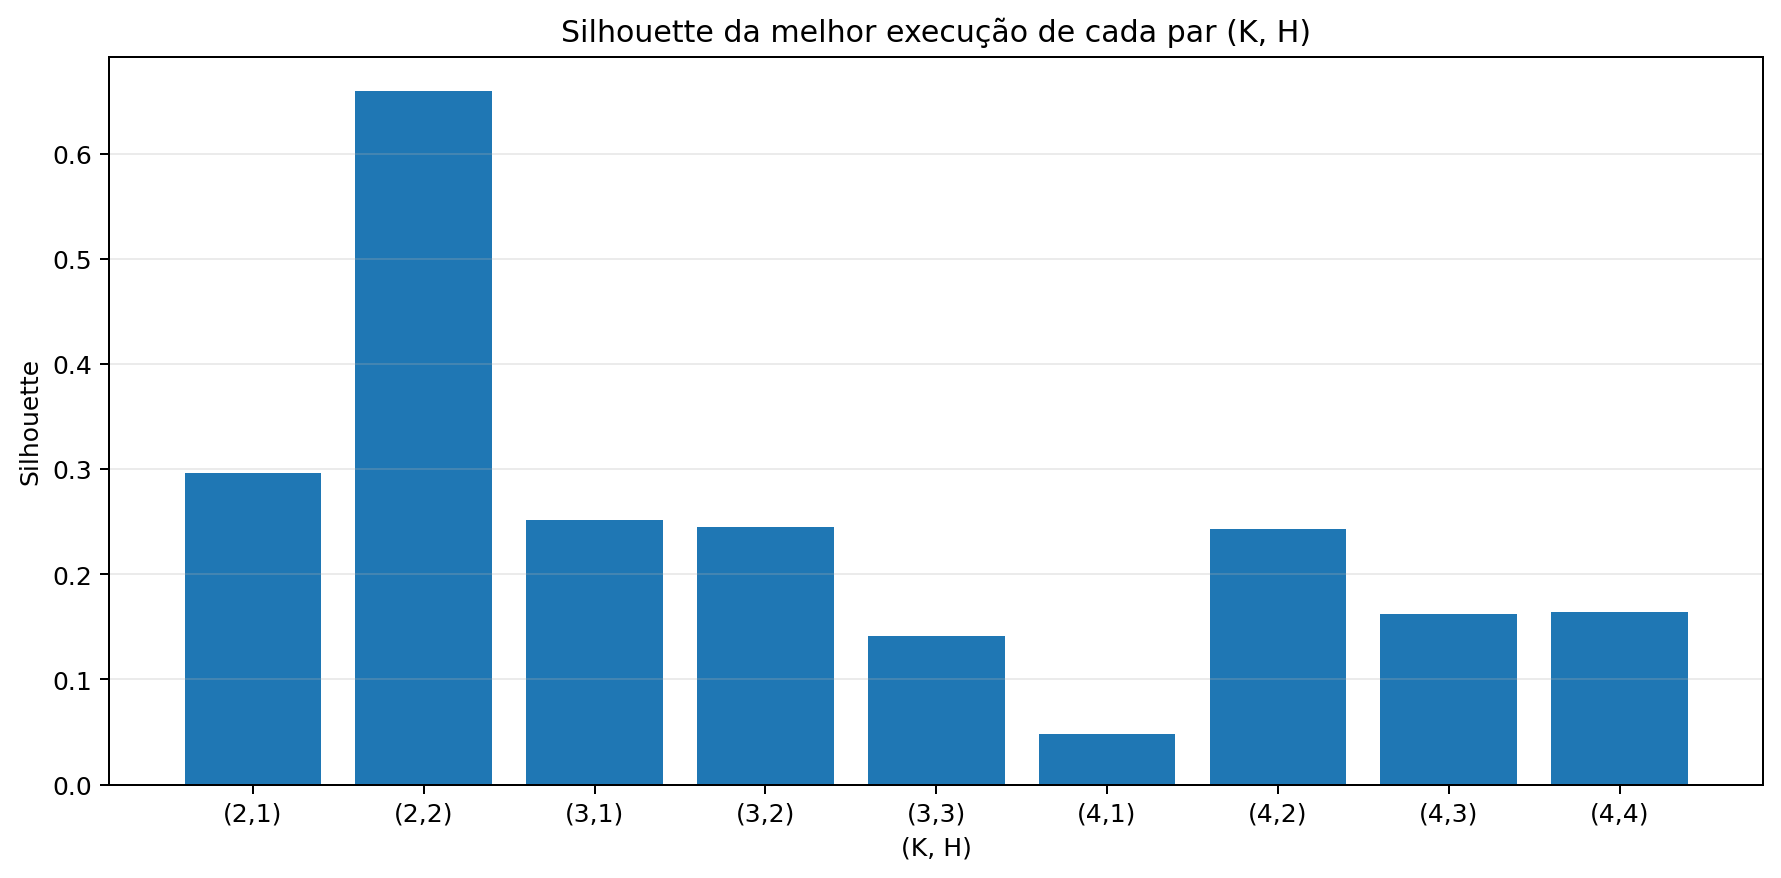
\includegraphics[width=\linewidth]{../questao1/resultados/revisada/silhouette_KH.png}
\par\smallskip\scriptsize Silhueta $\times$ $(K, H)$ --- Linha de Base (\texttt{revisada})
\end{minipage}\hfill
\begin{minipage}[t]{0.32\linewidth}
\centering
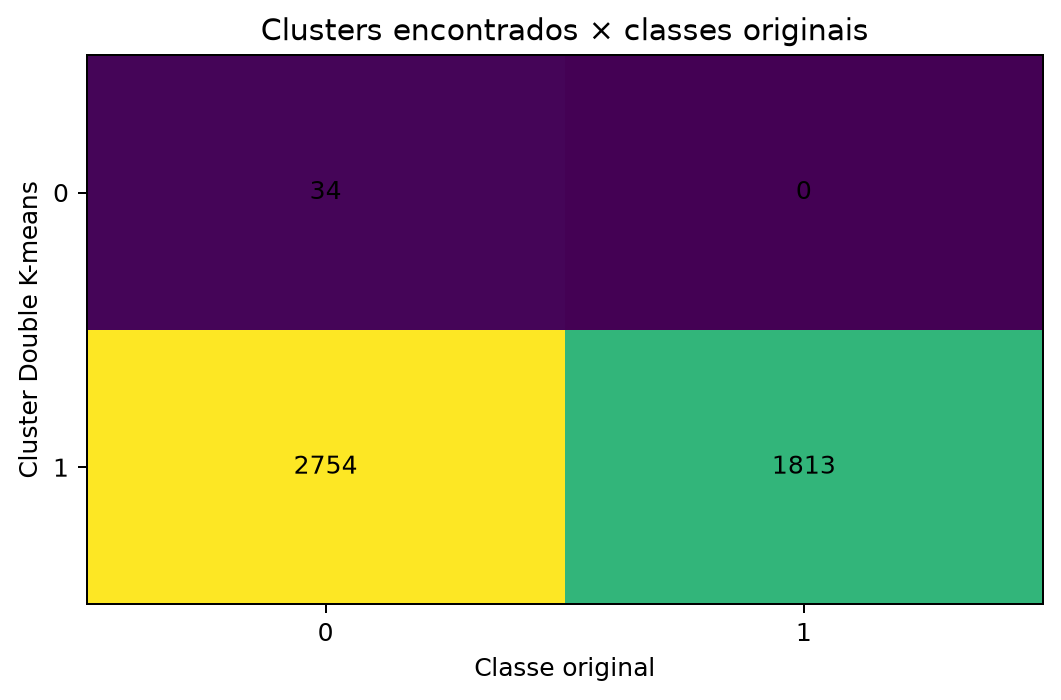
\includegraphics[width=\linewidth]{../questao1/resultados/revisada/matriz_contingencia.png}
\par\smallskip\scriptsize Contingência --- Linha de Base (\texttt{revisada})
\end{minipage}\hfill
\begin{minipage}[t]{0.32\linewidth}
\centering
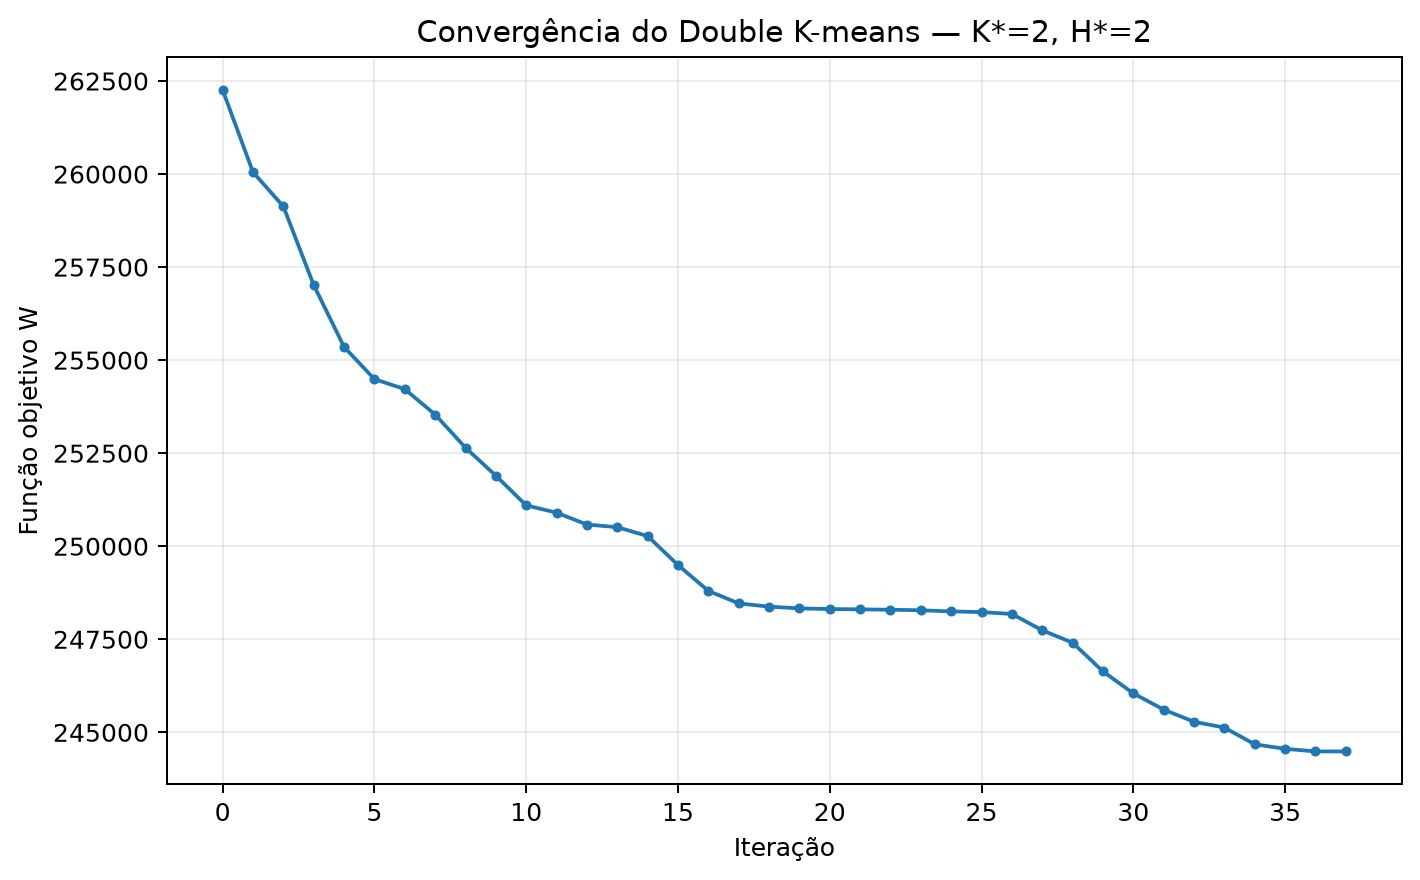
\includegraphics[width=\linewidth]{../questao1/resultados/revisada/objetivo_iteracoes.png}
\par\smallskip\scriptsize Convergência de $W$ --- Linha de Base (\texttt{revisada})
\end{minipage}
\captionof{figure}{Diagnóstico visual da estratégia linha de base (\texttt{revisada}): Silhueta, contingência e convergência de $W$.}
\end{minipage}
\end{center}


\subsubsection{\texorpdfstring{Solução Oficial Selecionada (\texttt{log\_minmax}): Co-clusters, Matriz G, Contingência e ARI}{Solução Oficial Selecionada (logminmax): Co-clusters, Matriz G, Contingência e ARI}}\label{sec:2-1-5-solucao-oficial-selecionada-logminmax-co-clusters-matriz-g-contingencia-e-ari}


A representação adotada pelo grupo para gerar a partição \texttt{y\_\allowbreak double\_\allowbreak kmeans} da Questão 2 foi \textbf{\texttt{log\_\allowbreak minmax}} ($\log(1+x)$ seguida de \texttt{MinMaxScaler}). Essa \textbf{decisão entre representações} combinou razões de tratamento dos dados (preservação das $57$ variáveis e compressão monotônica de caudas longas) com a concordância externa observada ($\text{ARI}=+0,391111$, maior entre as soluções vencedoras por Silhueta de cada representação). \textbf{O ARI não determinou $(K^*,H^*)=(3,3)$}: esse par foi selecionado pela maior Silhueta entre os nove pares \textbf{dentro de \texttt{log\_\allowbreak minmax}}. Como o ARI influenciou a escolha final da representação, essa decisão não foi inteiramente não supervisionada. A transformação logarítmica reduz a influência de valores extremos nas variáveis não negativas e a normalização coloca os $57$ atributos em uma escala comum, sem excluir colunas. Essas propriedades constituem uma justificativa técnica independente dos rótulos, mas, isoladamente, não demonstram que essa seja a melhor representação não supervisionada entre as sete avaliadas. Assim, o ARI de $+0,391111$ deve ser interpretado como evidência externa exploratória da solução escolhida, e não como validação independente de uma representação selecionada sem consultar as classes conhecidas:

\begin{itemize}[leftmargin=1.5em, itemsep=0.25em, topsep=0.25em]
  \item \textbf{Par ótimo escolhido:} $(K^*, H^*) = (3, 3)$, \texttt{best\_\allowbreak seed =\allowbreak  33044}, convergência em \textbf{$14$ iterações}, $W = 2.906,230738$, $\text{Silhueta} = 0,129219$, $\text{ARI} = +0,391111$ (houve $2$ tentativas inválidas descartadas antes de atingir $100$ rodadas válidas em $(3,3)$).
  \item \textbf{Partição das $57$ variáveis ($H^* = 3$)} (\texttt{particao\_\allowbreak variaveis.csv}):
\begin{itemize}[leftmargin=1.5em, itemsep=0.25em, topsep=0.25em]
  \item \textbf{Grupo de variáveis \texttt{0} ($4$ atributos):} \texttt{capital\_\allowbreak run\_\allowbreak length\_\allowbreak longest}, \texttt{capital\_\allowbreak run\_\allowbreak length\_\allowbreak total}, \texttt{word\_\allowbreak freq\_\allowbreak you}, \texttt{word\_\allowbreak freq\_\allowbreak your};
  \item \textbf{Grupo de variáveis \texttt{1} ($31$ atributos):} \texttt{char\_\allowbreak freq\_\allowbreak \#}, \texttt{(\allowbreak }, \texttt{;}, \texttt{[} e $27$ termos frequenciais, incluindo termos técnicos/contextuais como \texttt{1999}, \texttt{3d}, \texttt{415}, \texttt{650}, \texttt{85}, \texttt{857}, \texttt{conference}, \texttt{cs}, \texttt{data}, \texttt{direct}, \texttt{edu}, \texttt{font}, \texttt{george}, \texttt{hp}, \texttt{hpl}, \texttt{lab}, \texttt{labs}, \texttt{meeting}, \texttt{original}, \texttt{parts}, \texttt{pm}, \texttt{project}, \texttt{re}, \texttt{report}, \texttt{table}, \texttt{technology}, \texttt{telnet};
  \item \textbf{Grupo de variáveis \texttt{2} ($22$ atributos):} \texttt{capital\_\allowbreak run\_\allowbreak length\_\allowbreak average}, \texttt{char\_\allowbreak freq\_\allowbreak !}, \texttt{char\_\allowbreak freq\_\allowbreak \$} e $19$ termos frequentes em comunicações comerciais/gerais (\texttt{000}, \texttt{address}, \texttt{addresses}, \texttt{all}, \texttt{business}, \texttt{credit}, \texttt{email}, \texttt{free}, \texttt{internet}, \texttt{mail}, \texttt{make}, \texttt{money}, \texttt{order}, \texttt{our}, \texttt{over}, \texttt{people}, \texttt{receive}, \texttt{remove}, \texttt{will}).
\end{itemize}
  \item \textbf{Matriz de protótipos dos blocos $G$} (\texttt{matriz\_\allowbreak prototipos\_\allowbreak G.csv}, médias no espaço pré-processado $[0, 1]$):
\end{itemize}
\begin{center}
\begin{minipage}{\linewidth}
\centering
\captionof{table}{Matriz de protótipos $G$ na solução oficial (\texttt{log\_minmax}, $(K^*,H^*)=(3,3)$).}
\small
\setlength{\tabcolsep}{5pt}
\renewcommand{\arraystretch}{1.18}
\begin{tabular}{l c c c}
\toprule
\textbf{Grupo de Objetos} & \textbf{Variáveis \texttt{0} (4 atributos)} & \textbf{Variáveis \texttt{1} (31 atributos)} & \textbf{Variáveis \texttt{2} (22 atributos)} \\
\midrule
\textbf{Cluster 0 ($2.619$ objetos)} & 0,194479 & 0,022612 & 0,025559 \\
\textbf{Cluster 1 ($265$ objetos)} & 0,240859 & \textbf{0,132449} & 0,024273 \\
\textbf{Cluster 2 ($1.717$ objetos)} & \textbf{0,420265} & 0,008495 & \textbf{0,090361} \\
\bottomrule
\end{tabular}
\end{minipage}
\end{center}


\begin{itemize}[leftmargin=1.5em, itemsep=0.25em, topsep=0.25em]
  \item \textbf{Matriz de contingência frente à partição original} (\texttt{matriz\_\allowbreak contingencia.csv}):
\end{itemize}
\begin{center}
\begin{minipage}{\linewidth}
\centering
\captionof{table}{Matriz de contingência entre os co-clusters de \texttt{log\_minmax} e \texttt{y\_original}.}
\small
\sloppy
\setlength{\tabcolsep}{5pt}
\renewcommand{\arraystretch}{1.18}
\begin{tabularx}{\linewidth}{l r r r L}
\toprule
\textbf{Cluster (\texttt{y\_\allowbreak double\_\allowbreak kmeans})} & \textbf{Non-spam (\texttt{0})} & \textbf{Spam (\texttt{1})} & \textbf{Total} & \textbf{Perfil Observado} \\
\midrule
\textbf{Cluster \texttt{0}} & 2.218 & 401 & \textbf{2.619} ($56,92\%$) & $84,69\%$ \textit{non-spam} \\
\textbf{Cluster \texttt{1}} & 265 & 0 & \textbf{265} ($5,76\%$) & $100,00\%$ \textit{non-spam} \\
\textbf{Cluster \texttt{2}} & 305 & 1.412 & \textbf{1.717} ($37,32\%$) & $82,24\%$ \textit{spam} \\
\textbf{Total} & \textbf{2.788} & \textbf{1.813} & \textbf{4.601} ($100\%$) & $\text{ARI} = +0,391111$ \\
\bottomrule
\end{tabularx}
\end{minipage}
\end{center}


\begin{itemize}[leftmargin=1.5em, itemsep=0.25em, topsep=0.25em]
  \item \textbf{Comentário sobre o ARI:} um ARI de $+0,3911$ indica concordância externa parcial e substantivamente superior ao acaso ($\text{ARI} \approx 0$): o Cluster \texttt{2} concentra $77,88\%$ ($1.412 / 1.813$) dos \textit{spams} da base, com protótipo elevado nas variáveis de maiúsculas (\texttt{0,\allowbreak 4203}) e termos comerciais/exclamativos (\texttt{0,\allowbreak 0904}); o Cluster \texttt{0} concentra a maior parte dos e-mails legítimos ($79,56\%$ dos \textit{non-spams}, embora com $401$ \textit{spams} misturados); e o Cluster \texttt{1} ($265$ e-mails, $100\%$ \textit{non-spam}) exibe intensidade média mais alta no grupo de variáveis \texttt{1} (\texttt{0,\allowbreak 1324}). Ainda assim, como um algoritmo não supervisionado otimiza homogeneidade geométrica e não fronteiras de classe, não há correspondência exata $1$-para-$1$.
\end{itemize}
\begin{center}
\begin{minipage}{\linewidth}
\centering
\begin{minipage}[t]{0.32\linewidth}
\centering
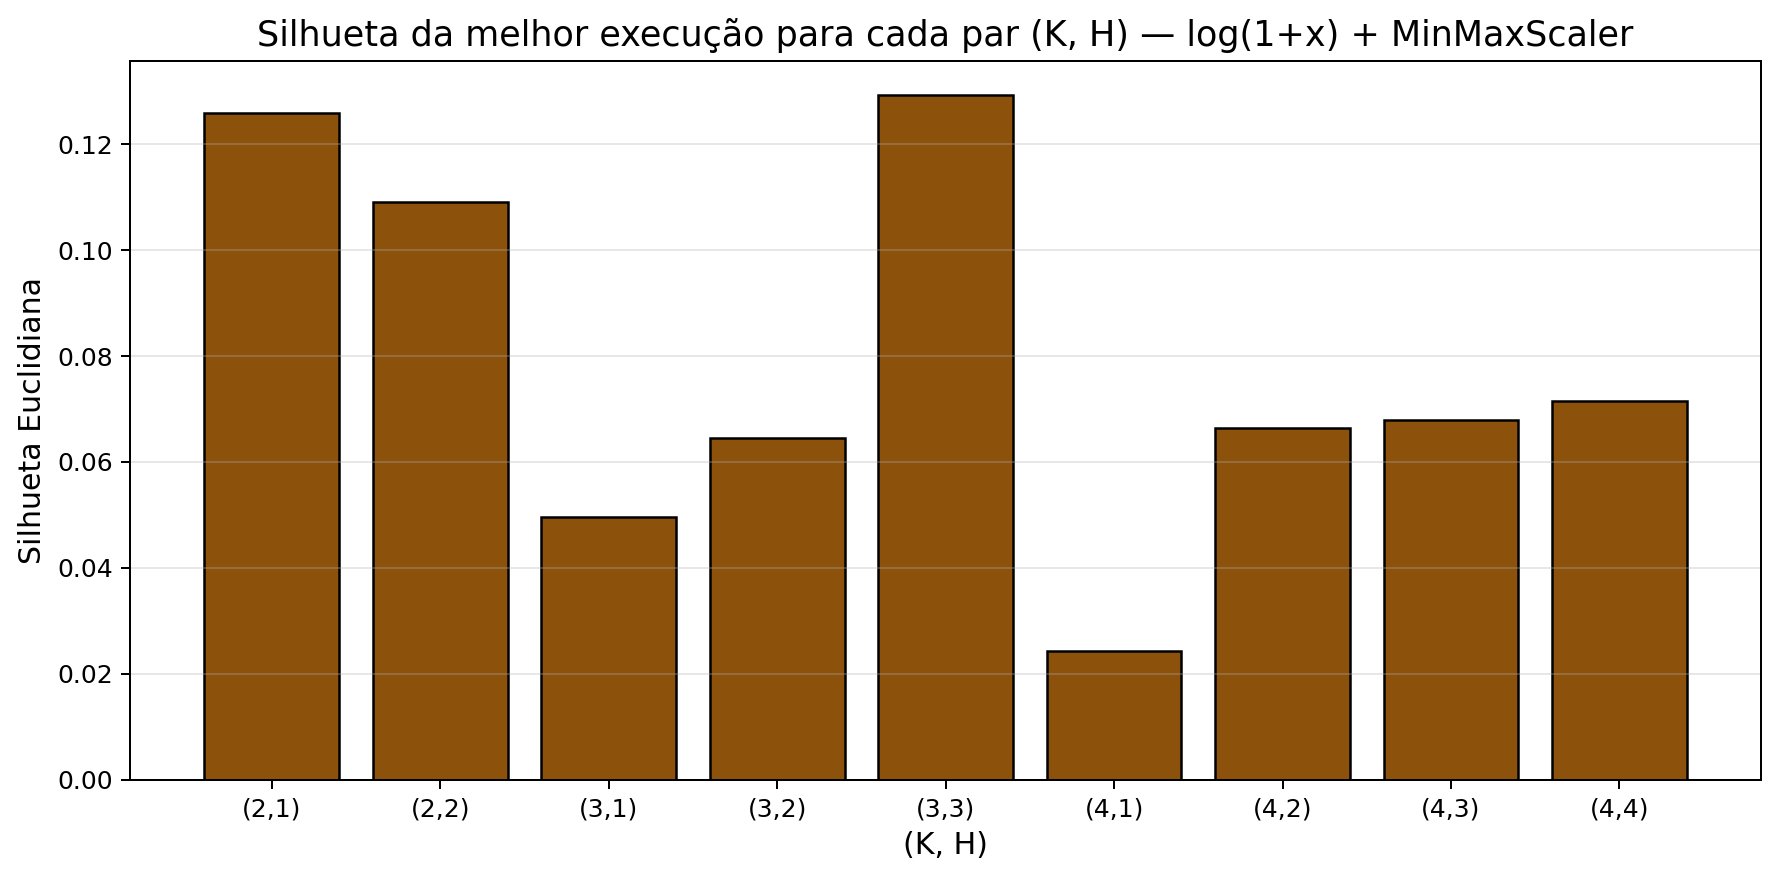
\includegraphics[width=\linewidth]{../questao1/resultados/log_minmax/silhouette_KH.png}
\par\smallskip\scriptsize Silhueta $\times$ $(K, H)$ --- Oficial (\texttt{log\_\allowbreak minmax})
\end{minipage}\hfill
\begin{minipage}[t]{0.32\linewidth}
\centering
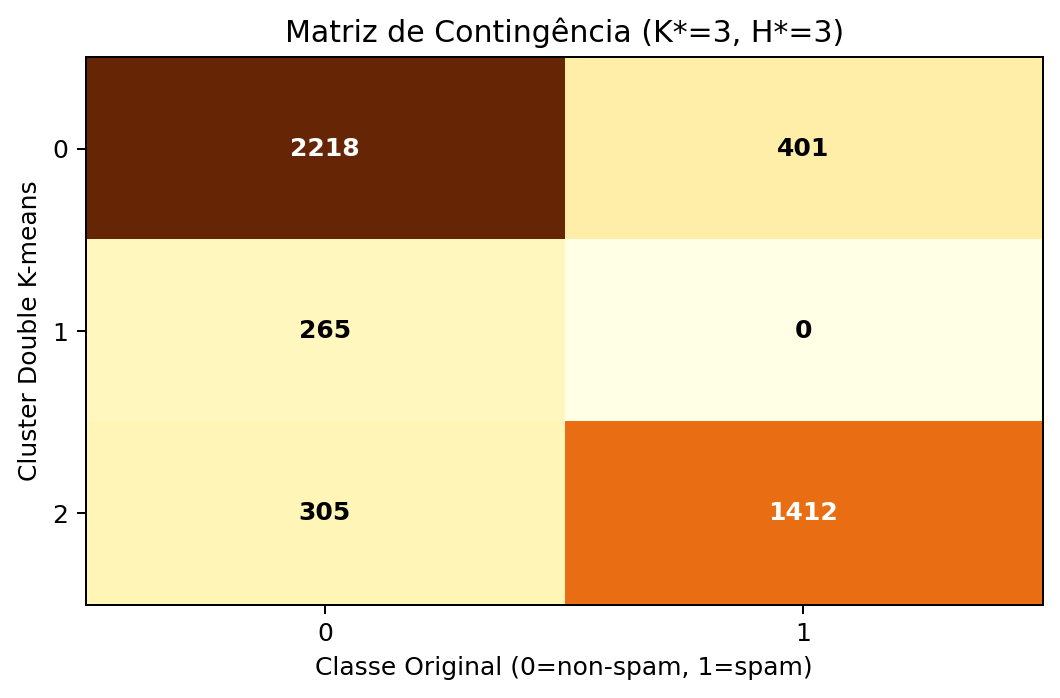
\includegraphics[width=\linewidth]{../questao1/resultados/log_minmax/matriz_contingencia.png}
\par\smallskip\scriptsize Contingência --- Oficial (\texttt{log\_\allowbreak minmax})
\end{minipage}\hfill
\begin{minipage}[t]{0.32\linewidth}
\centering
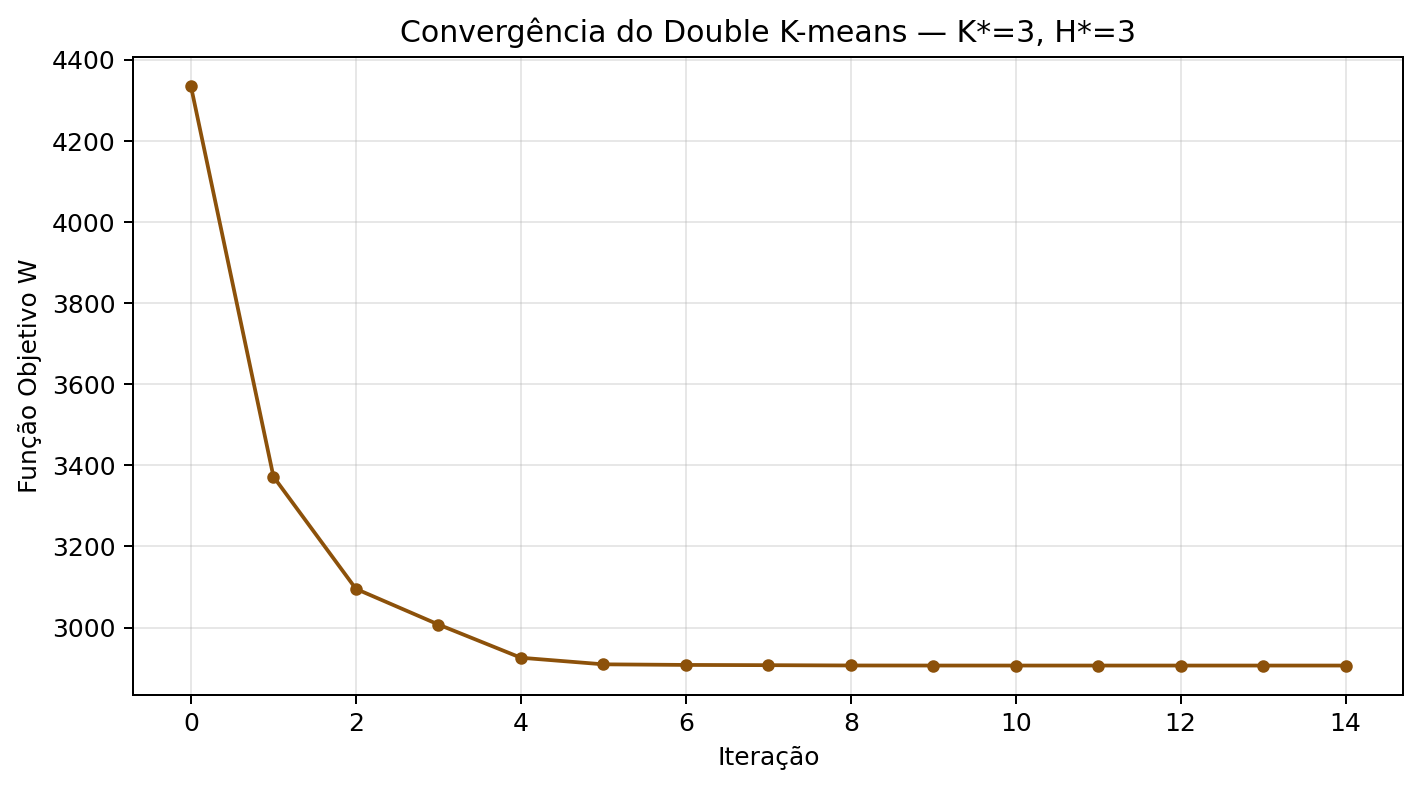
\includegraphics[width=\linewidth]{../questao1/resultados/log_minmax/objetivo_iteracoes.png}
\par\smallskip\scriptsize Convergência de $W$ --- Oficial (\texttt{log\_\allowbreak minmax})
\end{minipage}
\captionof{figure}{Diagnóstico visual da estratégia oficial (\texttt{log\_minmax}): Silhueta, contingência e convergência de $W$.}
\end{minipage}
\end{center}



\subsection{\texorpdfstring{Transição Segura entre Questão 1 e Questão 2 (Prevenção de \textit{Data Leakage})}{Transição Segura entre Questão 1 e Questão 2 (Prevenção de Data Leakage)}}\label{sec:2-2-transicao-segura-entre-questao-1-e-questao-2-prevencao-de-data-leakage}


A passagem da Questão 1 para a Questão 2 foi protegida por quatro barreiras metodológicas explícitas (\texttt{questao2/\allowbreak dados/\allowbreak proveniencia\_\allowbreak q1.json}, \texttt{questao2/\allowbreak src/\allowbreak dados.py}):

\begin{enumerate}[leftmargin=1.5em, itemsep=0.25em, topsep=0.25em]
  \item \textbf{Preservação da escala original:} o arquivo \texttt{questao2/\allowbreak dados/\allowbreak spambase\_\allowbreak q2.csv} é cópia verificada byte a byte de \texttt{spambase\_\allowbreak com\_\allowbreak clusters\_\allowbreak log\_\allowbreak minmax.csv} (SHA-256 \texttt{84d4176669d71313\allowbreak 8b584e354ac05060\allowbreak 25a21bae3dc16979\allowbreak 5ed78c745480eb4a}), contendo os $57$ atributos na \textbf{escala bruta original}, acrescidos das colunas \texttt{y\_\allowbreak original} e \texttt{y\_\allowbreak double\_\allowbreak kmeans}.
  \item \textbf{Isolamento por fold (\textit{Pipeline} aninhado):} na Questão 2, os quatro classificadores paramétricos/não paramétricos encapsulam \texttt{FunctionTransformer(\allowbreak np.log1p)} e \texttt{MinMaxScaler(\allowbreak )} em um \texttt{Pipeline} ajustado \textbf{exclusivamente} nos índices de treinamento de cada fold interno ($5$-fold) e depois no conjunto de treinamento externo ($9$ folds). O fold de teste recebe apenas \texttt{transform(\allowbreak )}.
  \item \textbf{Proibição de vazamento entre alvos:} ao treinar classificadores para \texttt{y\_\allowbreak original}, a coluna \texttt{y\_\allowbreak double\_\allowbreak kmeans} é completamente excluída; o inverso vale ao treinar para \texttt{y\_\allowbreak double\_\allowbreak kmeans}.
  \item \textbf{Distinção entre validade supervisionada e transdutiva:} os rótulos \texttt{y\_\allowbreak double\_\allowbreak kmeans} foram aprendidos pelo Double K-means sobre toda a matriz de $4.601$ instâncias na Questão 1. Por essa razão, os experimentos da Questão 2 sobre \texttt{y\_\allowbreak double\_\allowbreak kmeans} avaliam o quão bem cada classificador supervisionado consegue \textbf{reproduzir uma partição previamente descoberta}, não equivalendo a uma validação externa independente de novos clusters sobre e-mails inéditos.
\end{enumerate}

\subsection{Questão 2 --- Classificação Supervisionada e Comparação Estatística}\label{sec:2-3-questao-2-classificacao-supervisionada-e-comparacao-estatistica}


\subsubsection{\texorpdfstring{Organização Experimental: 30 $\times$ 10-Folds, Tuning 5-Folds Interno e Métricas}{Organização Experimental: 30 x 10-Folds, Tuning 5-Folds Interno e Métricas}}\label{sec:2-3-1-organizacao-experimental-30-10-folds-tuning-5-folds-interno-e-metricas}


Conforme \texttt{questao2/\allowbreak src/\allowbreak validacao.py} e \texttt{questao2/\allowbreak src/\allowbreak metricas.py}, o protocolo foi organizado separadamente para cada variável resposta (\texttt{y\_\allowbreak original} e \texttt{y\_\allowbreak double\_\allowbreak kmeans}):

\begin{itemize}[leftmargin=1.5em, itemsep=0.25em, topsep=0.25em]
  \item \textbf{Validação cruzada externa 30 $\times$ 10-folds:} executam-se $30$ repetições ($r = 1, \ldots, 30$) de \texttt{StratifiedKFold(\allowbreak n\_\allowbreak splits=\allowbreak 10,\allowbreak  shuffle=\allowbreak True,\allowbreak  random\_\allowbreak state=\allowbreak 2026 + r - 1)}. Em cada repetição, todas as $4.601$ instâncias são testadas exatamente uma vez sem sobreposição nem vazamento. Dentro de cada alvo, os cinco classificadores compartilham \textbf{exatamente os mesmos índices de treino e teste} em todas as $300$ partições externas ($30 \times 10$). Ao todo, foram auditadas \textbf{$3.000$ avaliações externas} ($10$ combinações alvo/modelo $\times 300$ folds) e \textbf{$1.380.300$ predições individuais out-of-fold} (\texttt{AUDITORIA\_\allowbreak 30x10.md}).
  \item \textbf{Validação cruzada interna 5-folds:} em cada fold externo $(rep, fold)$, os quatro classificadores-base realizam busca exaustiva em grade (\textit{grid search}) por \texttt{StratifiedKFold(\allowbreak n\_\allowbreak splits=\allowbreak 5,\allowbreak  shuffle=\allowbreak True,\allowbreak  random\_\allowbreak state=\allowbreak 2026 + 1000*rep + fold)} restrita aos $9$ folds de treino externo, maximizando o \textbf{F1 macro} médio de validação interna (\texttt{zero\_\allowbreak division=\allowbreak 0}). Selecionado o melhor conjunto de hiperparâmetros, o \texttt{Pipeline} correspondente é reajustado do zero nos $9$ folds de treino e avaliado uma única vez no $10^\circ$ fold de teste externo.
  \item \textbf{Métricas avaliadas:}
\begin{gather*}
\text{Taxa de erro} = 1 - \text{Acurácia}, \quad \text{Precisão}_{\text{macro}} = \frac{1}{C}\sum_{c=1}^{C} P_c, \\[0.4em] \text{Cobertura}_{\text{macro}} = \frac{1}{C}\sum_{c=1}^{C} R_c, \quad \text{F1}_{\text{macro}} = \frac{1}{C}\sum_{c=1}^{C} \frac{2 P_c R_c}{P_c + R_c}
\end{gather*}
O uso de médias \textbf{macro} é essencial porque o Cluster \texttt{1} de \texttt{y\_\allowbreak double\_\allowbreak kmeans} possui apenas $265$ e-mails ($5,76\%$); métricas ponderadas ou acurácia pura poderiam mascarar falhas nessa classe minoritária. Métricas por classe também são salvas por fold em todos os CSVs de resultado.
  \item \textbf{Estimativas pontuais e ICs:} a medida de cada repetição ($1 \ldots 30$) é a média aritmética dos seus $10$ folds externos; a estimativa pontual é a média das $30$ repetições. Os intervalos de $95\%$ utilizam a distribuição \textit{t} de Student ($gl = 29$) sobre essas $30$ médias, com \textbf{caráter explicitamente descritivo}, dado que as $30$ repetições reutilizam o mesmo conjunto de $4.601$ instâncias.
\end{itemize}
\subsubsection{Modelos Implementados e Obtenção dos Hiperparâmetros}\label{sec:2-3-2-modelos-implementados-e-obtencao-dos-hiperparametros}


A tabela abaixo resume a formulação de cada um dos cinco modelos, as grades avaliadas na CV interna $5$-folds e as frequências reais observadas nos \textbf{$300$ folds externos} de cada alvo (auditadas diretamente em \texttt{questao2/\allowbreak resultados/\allowbreak \{modelo\}/\allowbreak \{alvo\}\_\allowbreak 30x10\_\allowbreak folds.csv}).

\begin{center}
\begin{minipage}{\linewidth}
\centering
\captionof{table}{Modelos supervisionados implementados na Questão 2, espaços de busca e hiperparâmetros selecionados ($300$ folds).}
\scriptsize
\sloppy
\setlength{\tabcolsep}{2.5pt}
\renewcommand{\arraystretch}{1.18}
\begin{tabularx}{\linewidth}{P{2.25cm} L P{2.85cm} P{2.3cm} P{2.3cm}}
\toprule
\textbf{Classificador} & \textbf{Formulação e Detalhes de Implementação} & \textbf{Espaço de Hiperparâmetros (CV Interna 5-folds)} & \textbf{Seleção Observada em \texttt{y\_\allowbreak original} (300 folds)} & \textbf{Seleção Observada em \texttt{y\_\allowbreak double\_\allowbreak kmeans} (300 folds)} \\
\midrule
\textbf{Bayesiano Gaussiano Multivariado} (\texttt{bayes\_\allowbreak gaussiano.py}) & Prioris empíricas $\hat{P}(\omega_c)=n_c/n$, médias $\hat\mu_c$ e covariâncias \textbf{completas} de máxima verossimilhança $\hat\Sigma_{c,\mathrm{ML}}$, com divisor $n_c$ (\textit{não} Naive Bayes). Para as log-densidades (via Cholesky) usa $\Sigma_{c,\text{utilizada}}=\hat\Sigma_{c,\mathrm{ML}}+\lambda s_{\text{treino}}I$, com $s_{\text{treino}}$ calculado só no treinamento; \textbf{não é a covariância ML pura}. & Regularização isotrópica relativa:\newline \texttt{\ensuremath{\lambda} \ensuremath{\in} \{1e-6,\allowbreak  1e-4,\allowbreak  1e-2,\allowbreak  1e-1\}} ($4$ candidatos) & \texttt{0.1}: $224$ folds\newline \texttt{0.01}: $76$ folds & \texttt{0.1}: $300$ folds ($100\%$) \\
\textbf{Bayes k-vizinhos (k-NN)} (\texttt{bayes\_\allowbreak knn.py}) & Estima posterior $\hat{P}(\omega_c \mid x) = k_c / k$ pela fração de classes entre os $k$ vizinhos mais próximos (conforme notas de aula de Técnicas Não Paramétricas); em caso de empate, remove iterativamente o vizinho mais distante até haver vencedor único. & \texttt{k \ensuremath{\in} \{1,\allowbreak  3,\allowbreak  5,\allowbreak  7,\allowbreak  11,\allowbreak  15,\allowbreak  21\}} $\times$\newline \texttt{distancia \ensuremath{\in} \{euclidiana,\allowbreak  city\_\allowbreak block,\allowbreak  chebyshev\}} ($21$ candidatos) & \texttt{city\_\allowbreak block}: $160$, \texttt{euclidiana}: $140$, \texttt{chebyshev}: $0$;\newline \texttt{k}: \texttt{\{5: 154,\allowbreak  7: 104,\allowbreak  3: 25,\allowbreak  1: 9,\allowbreak  11: 8\}} & \texttt{euclidiana}: $289$, \texttt{city\_\allowbreak block}: $11$, \texttt{chebyshev}: $0$;\newline \texttt{k}: \texttt{\{1: 133,\allowbreak  7: 86,\allowbreak  3: 43,\allowbreak  5: 32,\allowbreak  11: 6\}} \\
\textbf{Bayes Parzen} (\texttt{bayes\_\allowbreak parzen.py}) & Estimador não paramétrico com kernel multivariado produto de gaussianas univariadas e largura única $h$ em \texttt{[log1p+MinMax]}: $\hat{p}(x \mid c) = \frac{1}{n_c} \sum_{i: y_i=c} \prod_{j=1}^{57} \frac{1}{h}\phi\!\left(\frac{x_j - x_{ij}}{h}\right)$, avaliado em escala logarítmica (\texttt{log-sum-exp}) em lotes. & Largura de janela:\newline \texttt{h \ensuremath{\in} \{0.04,\allowbreak  0.08,\allowbreak  0.12,\allowbreak  0.20,\allowbreak  0.35,\allowbreak  0.55\}} ($6$ candidatos) & \texttt{0.12}: $300$ folds ($100\%$) & \texttt{0.20}: $249$ folds\newline \texttt{0.12}: $51$ folds \\
\textbf{Regressão Logística} (\texttt{regressao\_\allowbreak logistica.py}) & Modelo linear discriminativo com penalidade L2 e otimizador L-BFGS (\texttt{max\_\allowbreak iter=\allowbreak 2000}, \texttt{tol=\allowbreak 1e-4}); utiliza perda \textit{softmax} multinomial para $3$ classes em vez de um-contra-todos. & \texttt{C \ensuremath{\in} \{0.03,\allowbreak  0.3,\allowbreak  3.0,\allowbreak  30.0,\allowbreak  300.0\}} $\times$\newline \texttt{class\_\allowbreak weight \ensuremath{\in} \{None,\allowbreak  'balanced'\}} ($10$ candidatos) & \texttt{C}: \texttt{\{30: 164,\allowbreak  300: 129,\allowbreak  3: 7\}};\newline \texttt{None}: $162$, \texttt{'balanced'}: $138$ & \texttt{C}: \texttt{\{300: 246,\allowbreak  30: 54\}};\newline \texttt{None}: $193$, \texttt{'balanced'}: $107$ \\
\textbf{Voto Majoritário} (\texttt{voto\_\allowbreak majoritario.py}) & Combina os rótulos preditos \textit{out-of-fold} pelos $4$ modelos anteriores nos mesmos índices de teste; em empates ($2 \times 2$ ou triplo/duplo em 3 classes), desempata pela maior priori estimada exclusivamente no treino externo. & Sem hiperparâmetros internos adicionais & Empates resolvidos por priori variaram de $7$ a $30$ instâncias por fold & Empates resolvidos por priori variaram de $8$ a $29$ instâncias por fold \\
\bottomrule
\end{tabularx}
\end{minipage}
\end{center}



\noindent\textbf{Ressalva sobre a especificação gaussiana.} Para cada classe $c$, a média e a covariância de máxima verossimilhança são
\[
\hat\mu_c=\frac{1}{n_c}\sum_{i:y_i=c}x_i,
\qquad
\hat\Sigma_{c,\mathrm{ML}}=\frac{1}{n_c}\sum_{i:y_i=c}(x_i-\hat\mu_c)(x_i-\hat\mu_c)^{\top}.
\]
A escala $s_{\text{treino}}$ é a média das variâncias dos $57$ atributos no conjunto de treinamento transformado, com divisor $n$, e não depende das observações do teste. Na avaliação oficial, o código acrescenta $\lambda s_{\text{treino}}I$ à matriz de cada classe, com $\lambda\in\{10^{-6},10^{-4},10^{-2},10^{-1}\}$ selecionado por validação cruzada interna de cinco folds. \textbf{Todos os candidatos oficiais têm $\lambda>0$}; portanto, a regularização foi utilizada em todos os ajustes, e não apenas em situações ocasionais de singularidade. Ela reduz o risco de instabilidade na decomposição de Cholesky e mantém termos fora da diagonal. Os resultados reportados são do \textbf{Gaussiano multivariado com covariância ML regularizada}.\par\noindent\textbf{Diagnóstico de estabilidade sem regularização.} Como verificação complementar, avaliou-se a possibilidade de utilizar $\lambda=0$ nos particionamentos da primeira repetição da validação cruzada, incluindo folds externos e internos. Foram examinadas $300$ matrizes de covariância ($120$ para os rótulos originais e $180$ para os rótulos do Double K-Means). Destas, $17$ e $60$, respectivamente, apresentaram posto numérico inferior a $57$. Com regularização nula, o ajuste completo foi concluído em apenas $9$ dos $10$ folds externos para os rótulos originais e em nenhum dos $10$ folds externos para os rótulos do Double K-Means; nos $50$ ajustes internos por alvo, houve $34$ e $0$ sucessos, respectivamente. Esses resultados evidenciam que a covariância ML sem regularização não oferece estabilidade suficiente para a implementação baseada em Cholesky. Assim, a regularização diagonal é uma decisão de estabilidade numérica tecnicamente motivada. O diagnóstico não demonstra que um valor específico de $\lambda$ seja ótimo: sua intensidade foi selecionada na CV interna, sem consultar os dados de teste.

\subsubsection{\texorpdfstring{Resultados da Avaliação 30 $\times$ 10-Folds (Estimativas Pontuais e ICs Descritivos)}{Resultados da Avaliação 30 x 10-Folds (Estimativas Pontuais e ICs Descritivos)}}\label{sec:2-3-3-resultados-da-avaliacao-30-10-folds-estimativas-pontuais-e-ics-descritivos}


Os valores abaixo reportam \textbf{média [IC95 inferior; IC95 superior]} (aproximação descritiva por \textit{t} de Student sobre as $30$ repetições, conforme \texttt{resumo\_\allowbreak metricas.csv} e \texttt{y\_\allowbreak double\_\allowbreak kmeans/\allowbreak resumo\_\allowbreak metricas.csv}).

\paragraph{\texorpdfstring{Versão 1 --- \texttt{y\_original} (\textit{spam} versus \textit{non-spam}, 2 classes)}{Versão 1 - yoriginal (spam versus non-spam, 2 classes)}}\mbox{}\\[-0.2em]\label{sec:versao-1-yoriginal-spam-versus-non-spam-2-classes}


\begin{center}
\begin{minipage}{\linewidth}
\centering
\captionof{table}{Resultados da avaliação $30 \times 10$-folds para \texttt{y\_original} (média e IC 95\%).}
\footnotesize
\sloppy
\setlength{\tabcolsep}{2.5pt}
\renewcommand{\arraystretch}{1.18}
\begin{tabularx}{\linewidth}{P{2.55cm} C C C C}
\toprule
\textbf{Classificador} & \textbf{Taxa de erro ($\downarrow$) [IC95]} & \textbf{Precisão macro ($\uparrow$) [IC95]} & \textbf{Cobertura macro ($\uparrow$) [IC95]} & \textbf{F1 macro ($\uparrow$) [IC95]} \\
\midrule
\textbf{Bayes gaussiano multivariado} & 15,16\% [15,11\%; 15,21\%] & 0,8525 [0,8520; 0,8529] & 0,8683 [0,8678; 0,8688] & 0,8471 [0,8466; 0,8476] \\
\textbf{Bayes k-vizinhos} & 6,74\% [6,67\%; 6,82\%] & 0,9321 [0,9313; 0,9329] & 0,9266 [0,9257; 0,9274] & 0,9290 [0,9282; 0,9298] \\
\textbf{Bayes Parzen} & 5,75\% [5,70\%; 5,81\%] & 0,9422 [0,9416; 0,9428] & \textbf{0,9372} [0,9366; 0,9378] & 0,9394 [0,9389; 0,9400] \\
\textbf{Regressão logística} & 6,16\% [6,12\%; 6,20\%] & 0,9357 [0,9352; 0,9361] & 0,9359 [0,9354; 0,9364] & 0,9355 [0,9351; 0,9360] \\
\textbf{Voto majoritário} & \textbf{5,71\%} [5,66\%; 5,76\%] & \textbf{0,9439} [0,9434; 0,9444] & 0,9364 [0,9358; 0,9370] & \textbf{0,9397} [0,9392; 0,9402] \\
\bottomrule
\end{tabularx}
\end{minipage}
\end{center}


\paragraph{\texorpdfstring{Versão 2 --- \texttt{y\_double\_kmeans} (3 clusters de objetos, $K^* = 3, H^* = 3$)}{Versão 2 - ydoublekmeans (3 clusters de objetos, K^ = 3, H^ = 3)}}\mbox{}\\[-0.2em]\label{sec:versao-2-ydoublekmeans-3-clusters-de-objetos-k-3-h-3}


\begin{center}
\begin{minipage}{\linewidth}
\centering
\captionof{table}{Resultados da avaliação $30 \times 10$-folds para \texttt{y\_double\_kmeans} (média e IC 95\%).}
\footnotesize
\sloppy
\setlength{\tabcolsep}{2.5pt}
\renewcommand{\arraystretch}{1.18}
\begin{tabularx}{\linewidth}{P{2.55cm} C C C C}
\toprule
\textbf{Classificador} & \textbf{Taxa de erro ($\downarrow$) [IC95]} & \textbf{Precisão macro ($\uparrow$) [IC95]} & \textbf{Cobertura macro ($\uparrow$) [IC95]} & \textbf{F1 macro ($\uparrow$) [IC95]} \\
\midrule
\textbf{Bayes gaussiano multivariado} & 16,99\% [16,93\%; 17,04\%] & 0,7624 [0,7616; 0,7632] & 0,8774 [0,8768; 0,8781] & 0,7976 [0,7968; 0,7984] \\
\textbf{Bayes k-vizinhos} & 6,55\% [6,46\%; 6,63\%] & 0,9392 [0,9376; 0,9408] & 0,8903 [0,8883; 0,8922] & 0,9114 [0,9099; 0,9129] \\
\textbf{Bayes Parzen} & 5,66\% [5,61\%; 5,71\%] & 0,9521 [0,9510; 0,9532] & 0,9000 [0,8990; 0,9011] & 0,9224 [0,9217; 0,9232] \\
\textbf{Regressão logística} & \textbf{0,95\%} [0,92\%; 0,98\%] & \textbf{0,9840} [0,9832; 0,9848] & \textbf{0,9819} [0,9810; 0,9828] & \textbf{0,9827} [0,9821; 0,9833] \\
\textbf{Voto majoritário} & 4,64\% [4,59\%; 4,69\%] & 0,9612 [0,9600; 0,9625] & 0,9141 [0,9129; 0,9153] & 0,9347 [0,9338; 0,9357] \\
\bottomrule
\end{tabularx}
\end{minipage}
\end{center}


\subsubsection{Comparação Estatística: Testes de Friedman e Pós-teste de Nemenyi}\label{sec:2-3-4-comparacao-estatistica-testes-de-friedman-e-pos-teste-de-nemenyi}


Seguindo \texttt{questao2/\allowbreak src/\allowbreak estatistica.py}, cada repetição $r \in \{1, \ldots, 30\}$ constitui um bloco pareado ($n = 30$ blocos; $k = 5$ classificadores) onde os modelos são ordenados da posição $1$ (melhor) à $5$ (pior). A diferença crítica de Nemenyi para $\alpha = 0,05$, $k = 5$ e $n = 30$ é \textbf{$\text{CD} = 1,1136$} ranks. Todos os resultados possuem caráter \textbf{exploratório}, pois os $30$ blocos compartilham as mesmas $4.601$ instâncias e o Voto Majoritário depende estruturalmente dos outros quatro modelos.

\paragraph{\texorpdfstring{Testes globais de Friedman ($n = 30$, $k = 5$, $\alpha = 0,05$, $\text{CD} = 1,1136$)}{Testes globais de Friedman (n = 30, k = 5, alpha = 0,05, textCD = 1,1136)}}\mbox{}\\[-0.2em]\label{sec:testes-globais-de-friedman-n-30-k-5-alpha-0-05-textcd-1-1136}


\begin{center}
\begin{minipage}{\linewidth}
\centering
\captionof{table}{Testes globais de Friedman ($n=30$, $k=5$, $\alpha=0{,}05$, $\text{CD}=1{,}1136$).}
\small
\setlength{\tabcolsep}{5pt}
\renewcommand{\arraystretch}{1.18}
\begin{tabular}{l l r r c}
\toprule
\textbf{Variável Resposta} & \textbf{Métrica} & \textbf{$\chi^2$ de Friedman} & \textbf{$p$-valor} & \textbf{Rejeita $H_0$?} \\
\midrule
\texttt{y\_\allowbreak original} & Taxa de erro & 114,5175 & \texttt{7,\allowbreak 91e-24} & Sim \\
\texttt{y\_\allowbreak original} & Precisão macro & 115,8933 & \texttt{4,\allowbreak 02e-24} & Sim \\
\texttt{y\_\allowbreak original} & Cobertura macro & 98,2400 & \texttt{2,\allowbreak 33e-20} & Sim \\
\texttt{y\_\allowbreak original} & F1 macro & 114,2400 & \texttt{9,\allowbreak 07e-24} & Sim \\
\texttt{y\_\allowbreak double\_\allowbreak kmeans} & Taxa de erro & 120,0000 & \texttt{5,\allowbreak 34e-25} & Sim \\
\texttt{y\_\allowbreak double\_\allowbreak kmeans} & Precisão macro & 120,0000 & \texttt{5,\allowbreak 34e-25} & Sim \\
\texttt{y\_\allowbreak double\_\allowbreak kmeans} & Cobertura macro & 119,2267 & \texttt{7,\allowbreak 81e-25} & Sim \\
\texttt{y\_\allowbreak double\_\allowbreak kmeans} & F1 macro & 120,0000 & \texttt{5,\allowbreak 34e-25} & Sim \\
\bottomrule
\end{tabular}
\end{minipage}
\end{center}


\paragraph{\texorpdfstring{Síntese dos Ranks Médios ($1 =$ melhor, $5 =$ pior) e Contrastes Principais de Nemenyi}{Síntese dos Ranks Médios (1 = melhor, 5 = pior) e Contrastes Principais de Nemenyi}}\mbox{}\\[-0.2em]\label{sec:sintese-dos-ranks-medios-1-melhor-5-pior-e-contrastes-principais-de-nemenyi}


\begin{itemize}[leftmargin=1.5em, itemsep=0.25em, topsep=0.25em]
  \item \textbf{Em \texttt{y\_\allowbreak original} (F1 macro):}
\begin{itemize}[leftmargin=1.5em, itemsep=0.25em, topsep=0.25em]
  \item Ranks médios: \textbf{Voto (\texttt{1,\allowbreak 40})}, \textbf{Parzen (\texttt{1,\allowbreak 60})}, \textbf{Logística (\texttt{3,\allowbreak 00})}, \textbf{k-NN (\texttt{4,\allowbreak 00})}, \textbf{Gaussiano (\texttt{5,\allowbreak 00})}.
  \item O contraste principal \textbf{Voto $\times$ Parzen} apresenta diferença de rank de apenas $0,20$ ($p = 0,988321$), logo o pós-teste \textbf{não detecta diferença} entre eles (o mesmo padrão se repete em Taxa de erro com $p = 0,9792$, Precisão macro com $p = 0,4761$ e Cobertura macro com $p = 0,9883$). Em Cobertura macro, Parzen (\texttt{1,\allowbreak 73}), Voto (\texttt{1,\allowbreak 93}) e Logística (\texttt{2,\allowbreak 33}) também não se distinguem estatisticamente pelo Nemenyi ($p \ge 0,5823$).
  \item Entre \textbf{Gaussiano (\texttt{5,\allowbreak 00})} e \textbf{k-NN (\texttt{4,\allowbreak 00})}, a diferença exata de $1,00$ rank fica abaixo de $\text{CD} = 1,1136$ ($p = 0,102449$ em Erro, Cobertura e F1; $p = 0,0838$ em Precisão), ilustrando que testes baseados exclusivamente em postos não capturam automaticamente a magnitude absoluta da diferença de médias ($\Delta \text{F1} \approx 0,0819$).
\end{itemize}
  \item \textbf{Em \texttt{y\_\allowbreak double\_\allowbreak kmeans} (F1 macro, Erro e Precisão macro):}
\begin{itemize}[leftmargin=1.5em, itemsep=0.25em, topsep=0.25em]
  \item Ranks médios exatos e idênticos nessas três métricas: \textbf{Logística (\texttt{1,\allowbreak 00})}, \textbf{Voto (\texttt{2,\allowbreak 00})}, \textbf{Parzen (\texttt{3,\allowbreak 00})}, \textbf{k-NN (\texttt{4,\allowbreak 00})}, \textbf{Gaussiano (\texttt{5,\allowbreak 00})} ($\chi^2 = 120,00$, concordância perfeita de ordenação nas $30$ repetições). Em Cobertura macro, apenas \texttt{k-NN} (\texttt{3,\allowbreak 97}) e \texttt{Parzen} (\texttt{3,\allowbreak 03}) oscilam em uma repetição ($\chi^2 = 119,23$).
  \item Embora a \textbf{Regressão Logística} lidere com ampla vantagem numérica ($\Delta \text{F1} = +0,0480$ sobre o Voto; erro $5 \times$ menor), pares adjacentes diferem por $1,00 < \text{CD} = 1,1136$ e têm $p = 0,102449$ no Nemenyi (\texttt{Logística \ensuremath{\times} Voto}, \texttt{Voto \ensuremath{\times} Parzen}, \texttt{Parzen \ensuremath{\times} k-NN}, \texttt{k-NN \ensuremath{\times} Gaussiano}). Já todos os pares separados por $2$ ou mais ranks --- como \texttt{Logística \ensuremath{\times} Parzen} ($p = 9,54 \times 10^{-6}$), \texttt{Logística \ensuremath{\times} k-NN} ($p = 2,00 \times 10^{-12}$) e \texttt{Logística \ensuremath{\times} Gaussiano} ($p = 1,11 \times 10^{-16}$) --- são detectados como significativamente distintos. (As tabelas integrais de todas as $4$ métricas encontram-se no \hyperref[sec:anexo-b-tabelas-completas-de-ranks-medios-e-pos-teste-de-nemenyi-todas-as-metricas]{Anexo B}.)
\end{itemize}
\end{itemize}
\subsubsection{Curvas de Aprendizagem (5\% a 95\%, passo 5\%)}\label{sec:2-3-5-curvas-de-aprendizagem-5-a-95-passo-5}


As curvas de aprendizagem foram produzidas separadamente da validação cruzada $30 \times 10$-folds, utilizando a base completa de $4.601$ observações. Para cada conjunto de rótulos, foram consideradas $19$ proporções de treinamento e teste, variando de $5\%/95\%$ a $95\%/5\%$, com incrementos de cinco pontos percentuais. Em cada proporção, realizou-se uma divisão estratificada e complementar dos dados, sem sobreposição entre os conjuntos de treinamento e teste, utilizando a semente $2026$.

Ao todo, foram realizadas $38$ divisões ($19$ proporções para cada conjunto de rótulos) e $190$ avaliações de classificadores, considerando os quatro modelos-base e o classificador por voto majoritário. Os cinco classificadores compartilharam os mesmos índices de treinamento e teste em cada divisão. O ajuste de hiperparâmetros, por meio de validação cruzada interna de cinco folds, e o pré-processamento com \texttt{log1p + MinMaxScaler} foram realizados exclusivamente sobre os dados de treinamento, evitando vazamento de informações do conjunto de teste. Para cada proporção, foram calculados os valores de F1 macro nos conjuntos de treinamento e teste. As amostras utilizadas nos diferentes percentuais não são necessariamente aninhadas.

\begin{center}
\begin{minipage}{\linewidth}
\centering
\captionof{table}{Resumo das curvas de aprendizagem (F1 macro Treino / Teste em 5\%, 25\%, 50\%, 75\% e 95\%).}
\footnotesize
\sloppy
\setlength{\tabcolsep}{2.5pt}
\renewcommand{\arraystretch}{1.18}
\begin{tabularx}{\linewidth}{P{2.25cm} l C C C C C}
\toprule
\textbf{Alvo} & \textbf{Classificador} & \textbf{F1 (5\% Tr / Te)} & \textbf{F1 (25\% Tr / Te)} & \textbf{F1 (50\% Tr / Te)} & \textbf{F1 (75\% Tr / Te)} & \textbf{F1 (95\% Tr / Te)} \\
\midrule
\textbf{\texttt{y\_\allowbreak original}} & Bayes gaussiano & 0,9378 / 0,8670 & 0,8646 / 0,8454 & 0,8517 / 0,8464 & 0,8484 / 0,8623 & 0,8494 / 0,8388 \\
\textbf{\texttt{y\_\allowbreak original}} & Bayes k-vizinhos & 0,9356 / 0,8455 & 0,9311 / 0,8937 & 0,9369 / 0,9105 & 0,9408 / 0,9236 & 0,9993 / 0,9086 \\
\textbf{\texttt{y\_\allowbreak original}} & Bayes Parzen & 0,9770 / 0,8618 & 0,9761 / 0,9012 & 0,9941 / 0,9237 & 0,9936 / 0,9271 & 0,9930 / 0,9082 \\
\textbf{\texttt{y\_\allowbreak original}} & Regressão logística & 0,9633 / \textbf{0,9092} & 0,9441 / \textbf{0,9320} & 0,9411 / \textbf{0,9395} & 0,9409 / 0,9301 & 0,9401 / \textbf{0,9280} \\
\textbf{\texttt{y\_\allowbreak original}} & Voto majoritário & 0,9771 / 0,8824 & 0,9538 / 0,9129 & 0,9638 / 0,9323 & 0,9585 / \textbf{0,9352} & 0,9851 / 0,9218 \\
\textbf{\texttt{y\_\allowbreak double\_\allowbreak kmeans}} & Bayes gaussiano & 0,9746 / 0,8143 & 0,8541 / 0,8069 & 0,8373 / 0,8088 & 0,8244 / 0,7797 & 0,8171 / 0,7484 \\
\textbf{\texttt{y\_\allowbreak double\_\allowbreak kmeans}} & Bayes k-vizinhos & 0,8826 / 0,8597 & 0,9368 / 0,8891 & 1,0000 / 0,9069 & 1,0000 / 0,9262 & 0,9411 / 0,8960 \\
\textbf{\texttt{y\_\allowbreak double\_\allowbreak kmeans}} & Bayes Parzen & 1,0000 / 0,8614 & 0,9994 / 0,8972 & 0,9948 / 0,9274 & 0,9869 / 0,9302 & 0,9865 / 0,9440 \\
\textbf{\texttt{y\_\allowbreak double\_\allowbreak kmeans}} & Regressão logística & 1,0000 / \textbf{0,9050} & 0,9972 / \textbf{0,9679} & 0,9997 / \textbf{0,9809} & 0,9998 / \textbf{0,9811} & 0,9966 / \textbf{0,9936} \\
\textbf{\texttt{y\_\allowbreak double\_\allowbreak kmeans}} & Voto majoritário & 0,9968 / 0,8648 & 0,9914 / 0,9100 & 0,9971 / 0,9364 & 0,9966 / 0,9498 & 0,9855 / 0,9440 \\
\bottomrule
\end{tabularx}
\end{minipage}
\end{center}


\textbf{Análise dos padrões observados:}
\begin{enumerate}[leftmargin=1.5em, itemsep=0.25em, topsep=0.25em]
  \item \textbf{Eficiência amostral da Regressão Logística:} já com $5\%$ de treinamento ($230$ amostras), alcança F1 de teste de $0,9092$ (\texttt{y\_\allowbreak original}) e $0,9050$ (\texttt{y\_\allowbreak double\_\allowbreak kmeans}), escalando suavemente para $0,9936$ aos $95\%$ em \texttt{y\_\allowbreak double\_\allowbreak kmeans} --- o que confirma que a partição induzida pelo Double K-means no espaço \texttt{log1p + MinMax} possui fronteiras altamente separáveis por hiperplanos lineares.
  \item \textbf{Lacuna treino--teste e memorização local:} em k-NN (quando a CV interna escolhe $k=1$) e em Parzen (com $h$ pequeno, como $0,12$), o F1 de treinamento atinge $0,99$ a $1,00$ porque o próprio exemplo de consulta contribui para sua vizinhança/densidade \textit{in-sample}; já o F1 de teste cresce progressivamente de $\sim 0,85$ ($5\%$) até $\sim 0,92\text{--}0,94$ ($75\%\text{--}90\%$).
  \item \textbf{Comportamento do Bayesiano Gaussiano:} com $5\%$ de treino ($230$ amostras em $57$ dimensões, matriz de covariância $57 \times 57$ estimada por classe), há forte sobreajuste inicial em treino ($0,9378$ em \texttt{y\_\allowbreak original} e $0,9746$ em \texttt{y\_\allowbreak double\_\allowbreak kmeans}), que cai para $\sim 0,85$ e $\sim 0,82$ à medida que $N_{\text{treino}}$ aumenta e reduz a variância amostral; em \texttt{y\_\allowbreak double\_\allowbreak kmeans}, o teste oscila até $0,7484$ em $95\%$ (com apenas $231$ amostras de teste, sendo cerca de $13$ na classe minoritária), não caracterizando prova de degradação real por ter sido usada uma única partição por percentual.
  \item \textbf{Oscilações em proporções elevadas:} aos $95\%$ de treino, restam apenas $231$ instâncias de teste e as divisões entre percentuais não são necessariamente aninhadas; logo, pequenas quedas pontuais em $95\%$ refletem variância amostral de um conjunto de teste pequeno.
\end{enumerate}
\begin{center}
\begin{minipage}{\linewidth}
\centering
\begin{minipage}[t]{0.48\linewidth}
\centering
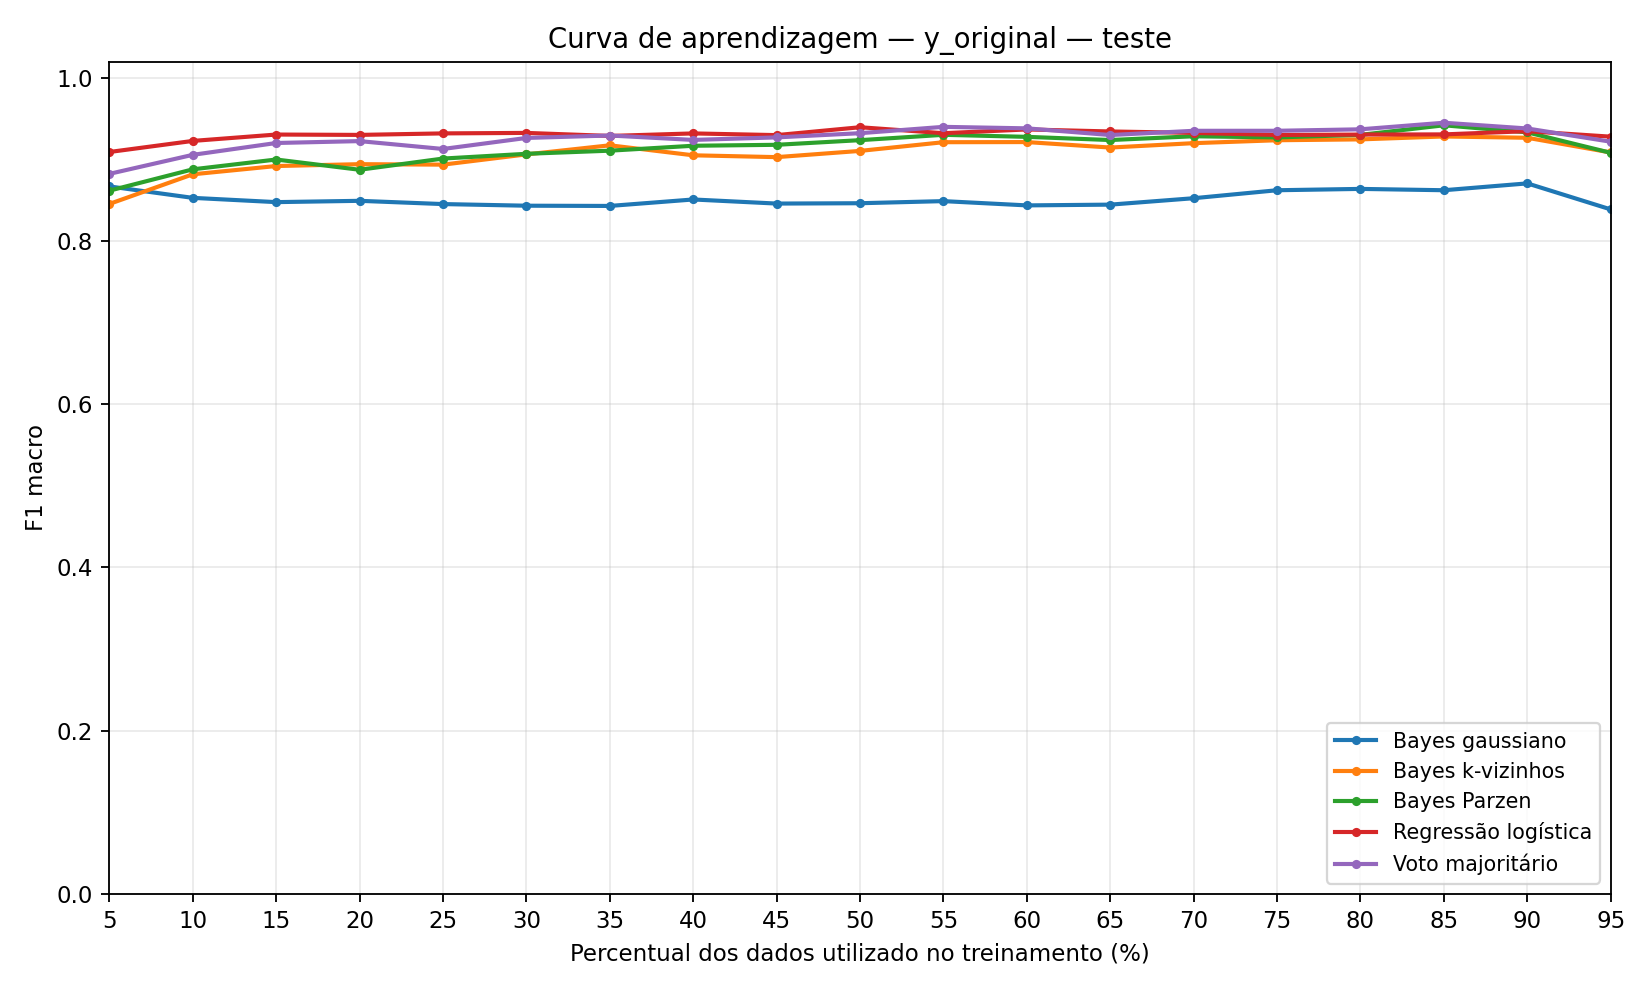
\includegraphics[width=\linewidth]{../questao2/resultados/curvas_aprendizagem/graficos/y_original_f1_teste.png}
\par\smallskip\scriptsize \texttt{y\_\allowbreak original} --- F1 Teste
\end{minipage}\hfill
\begin{minipage}[t]{0.48\linewidth}
\centering
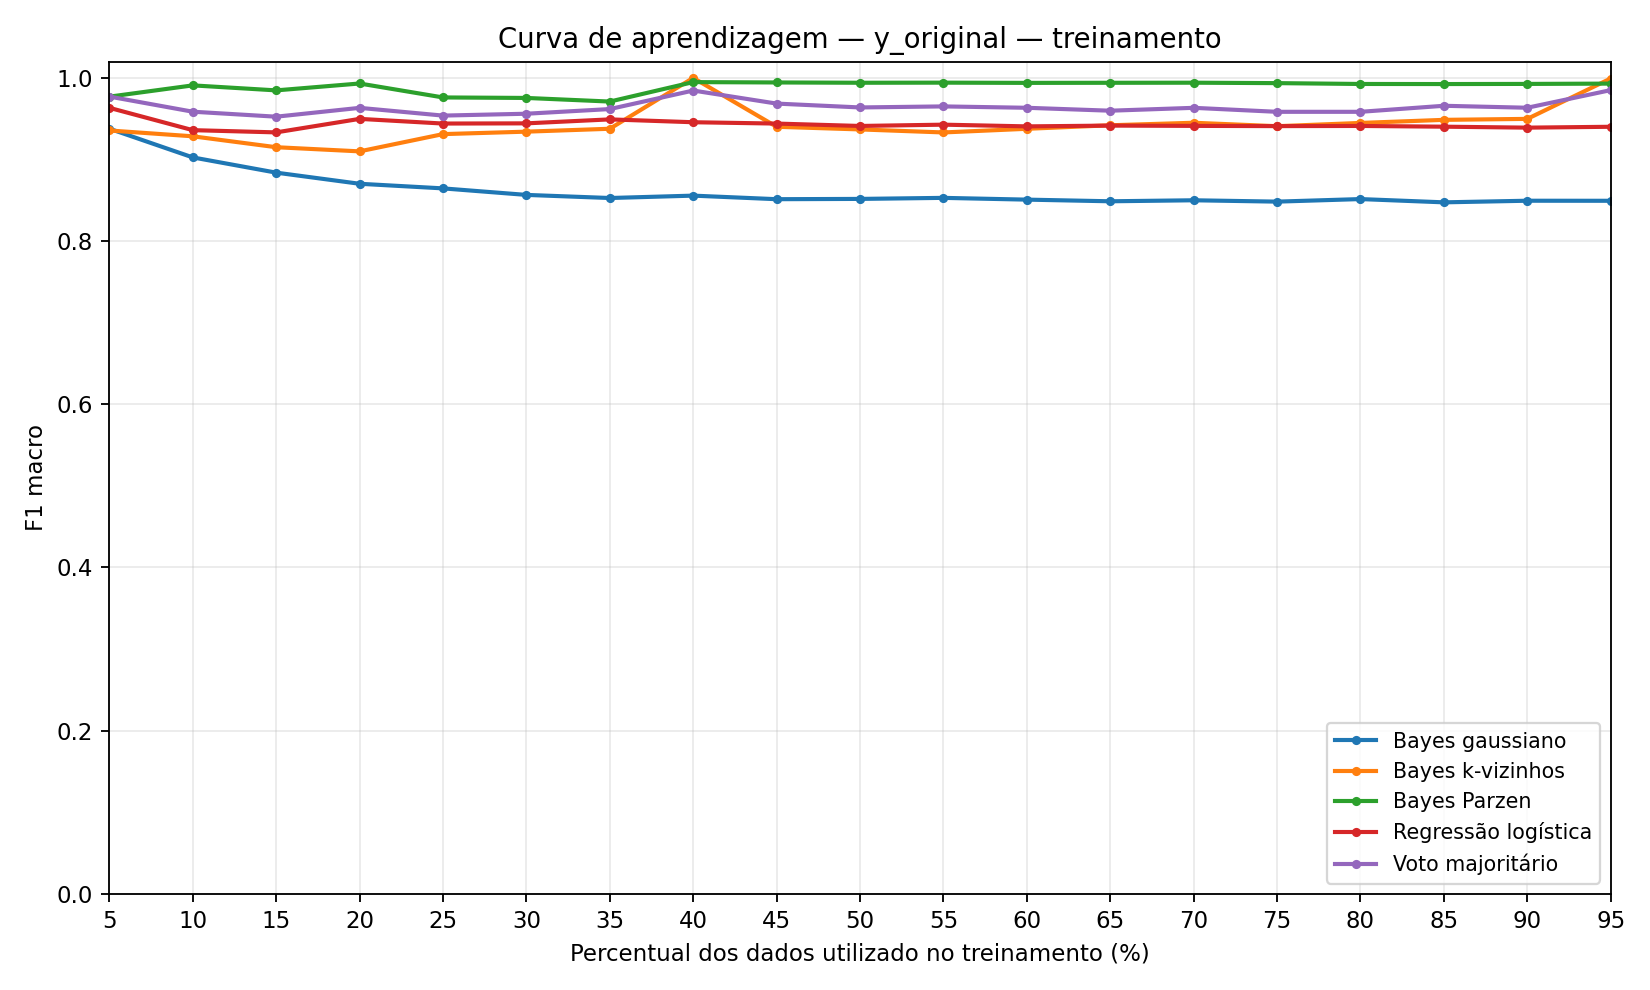
\includegraphics[width=\linewidth]{../questao2/resultados/curvas_aprendizagem/graficos/y_original_f1_treinamento.png}
\par\smallskip\scriptsize \texttt{y\_\allowbreak original} --- F1 Treinamento
\end{minipage}
\par\medskip
\begin{minipage}[t]{0.48\linewidth}
\centering
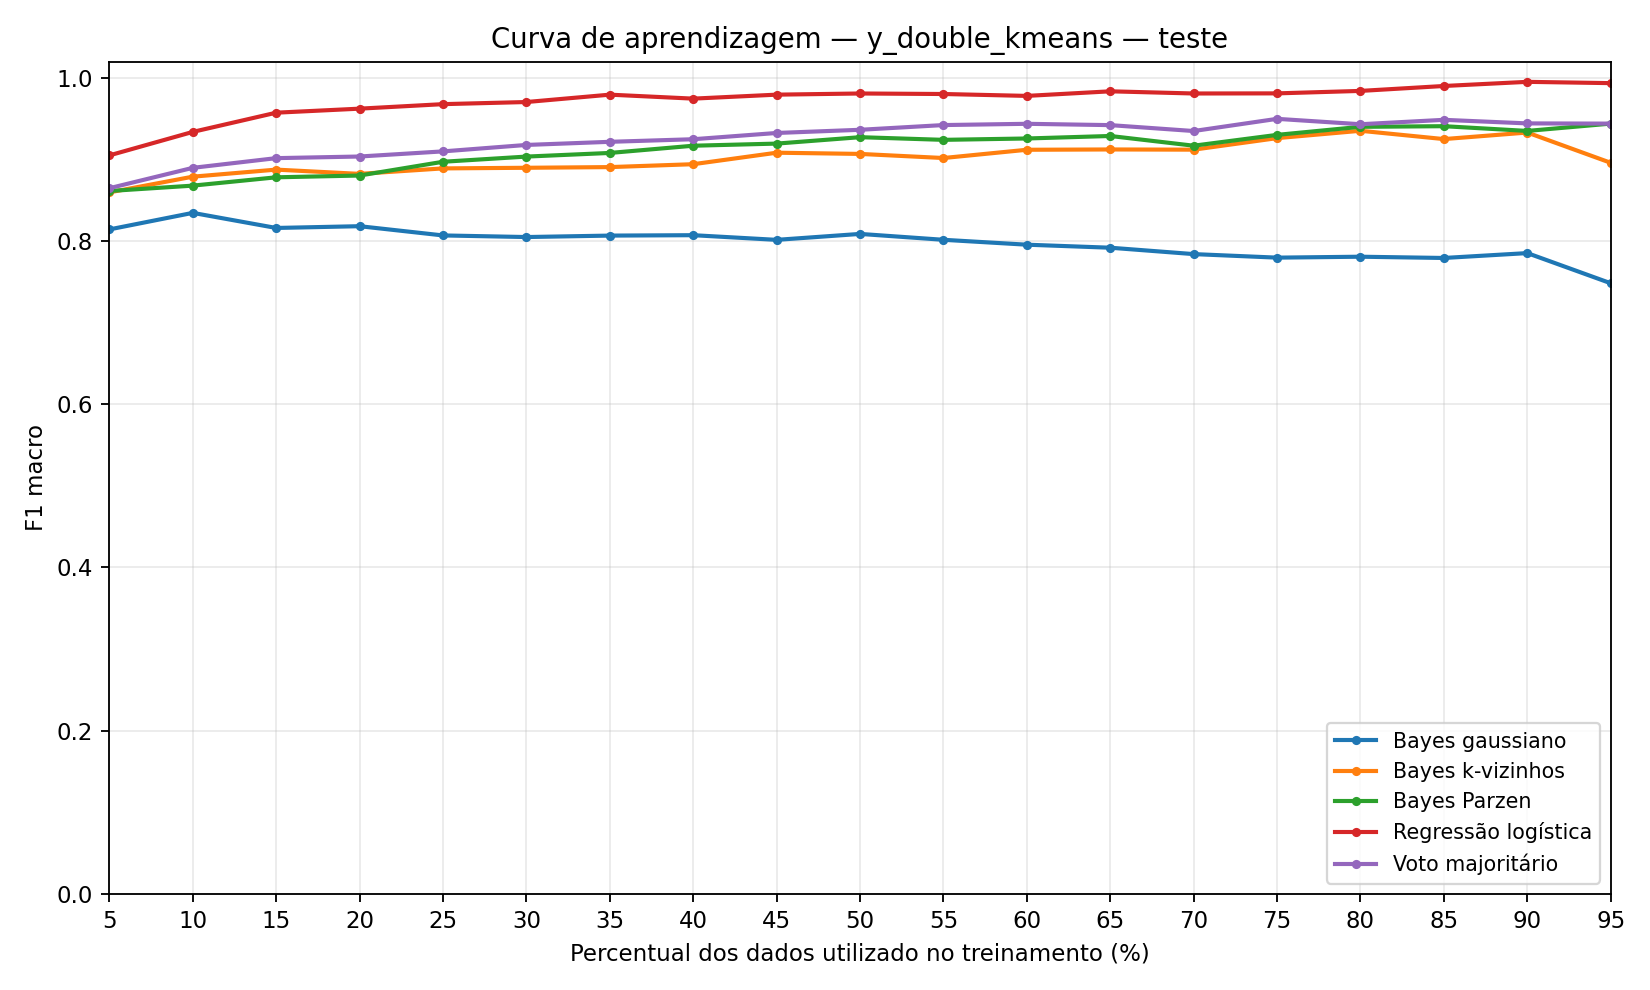
\includegraphics[width=\linewidth]{../questao2/resultados/curvas_aprendizagem/graficos/y_double_kmeans_f1_teste.png}
\par\smallskip\scriptsize \textbf{\texttt{y\_\allowbreak double\_\allowbreak kmeans} --- F1 Teste}
\end{minipage}\hfill
\begin{minipage}[t]{0.48\linewidth}
\centering
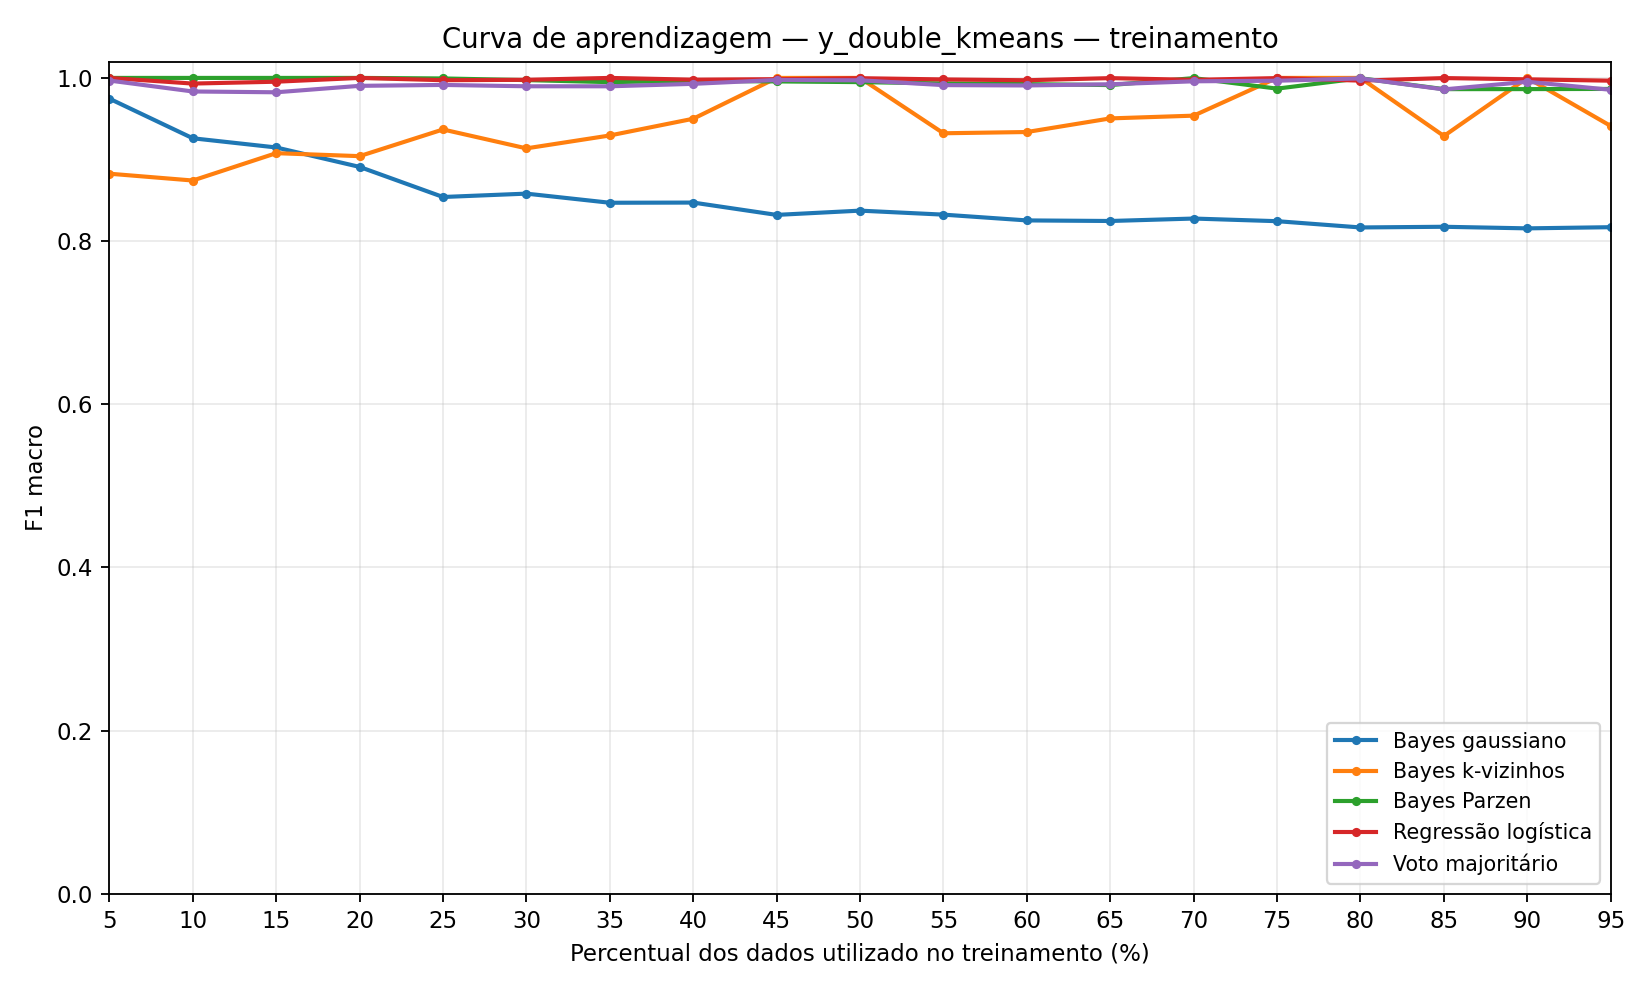
\includegraphics[width=\linewidth]{../questao2/resultados/curvas_aprendizagem/graficos/y_double_kmeans_f1_treinamento.png}
\par\smallskip\scriptsize \textbf{\texttt{y\_\allowbreak double\_\allowbreak kmeans} --- F1 Treinamento}
\end{minipage}
\captionof{figure}{Curvas de aprendizagem (F1 macro, $5\%$ a $95\%$ de treinamento) em teste e treinamento para \texttt{y\_original} e \texttt{y\_double\_kmeans}.}
\end{minipage}
\end{center}


\subsubsection{Estudo Complementar de Sensibilidade ao Pré-processamento}\label{sec:2-3-6-estudo-complementar-de-sensibilidade-ao-pre-processamento}


Sem alterar nem substituir a avaliação oficial $30 \times 10$-folds, conduziu-se em \texttt{questao2/\allowbreak scripts/\allowbreak comparar\_\allowbreak preprocessamento.py} uma comparação pareada de $1 \times 10$-folds ($300$ avaliações externas: $2$ alvos $\times 3$ estratégias $\times 5$ modelos $\times 10$ folds, com ajustes internos $5$-fold), incluindo uma reavaliação (\texttt{v2}, $80$ registros) que elevou \texttt{max\_\allowbreak iter=\allowbreak 20000,\allowbreak  tol=\allowbreak 1e-6} na Logística em escala bruta (reduzindo avisos de não convergência de $311 \to 171$ em \texttt{y\_\allowbreak original} e $510 \to 308$ em \texttt{y\_\allowbreak double\_\allowbreak kmeans}, sem eliminá-los) e ampliou a grade de Parzen em \texttt{MinMax} puro para $h \in \{0,005; 0,01; 0,02; 0,03; 0,04; 0,08; 0,12; 0,20; 0,35; 0,55\}$ (\texttt{comparacao\_\allowbreak resumo.csv}):

\begin{center}
\begin{minipage}{\linewidth}
\centering
\captionof{table}{Estudo complementar de sensibilidade ao pré-processamento na Questão 2 ($1 \times 10$-folds, F1 macro).}
\footnotesize
\sloppy
\setlength{\tabcolsep}{2.5pt}
\renewcommand{\arraystretch}{1.18}
\begin{tabularx}{\linewidth}{P{2.25cm} P{2.85cm} C C C C}
\toprule
\textbf{Alvo} & \textbf{Classificador} & \textbf{Sem Pré-processamento} & \textbf{Apenas MinMax} & \textbf{\texttt{Log1p + MinMax}} & \textbf{Ganho (\texttt{Log1p+MinMax} vs Bruto)} \\
\midrule
\texttt{y\_\allowbreak original} & Gaussiano multivariado & 0,8279 & 0,8287 & \textbf{0,8467} & +0,0188 \\
\texttt{y\_\allowbreak original} & Bayes k-vizinhos & 0,8445 & 0,9054 & \textbf{0,9287} & +0,0842 \\
\texttt{y\_\allowbreak original} & Bayes Parzen & 0,8268 & 0,9022 & \textbf{0,9416} & +0,1148 \\
\texttt{y\_\allowbreak original} & Regressão logística & 0,9247 & 0,9230 & \textbf{0,9352} & +0,0105 \\
\texttt{y\_\allowbreak original} & Voto majoritário & 0,8937 & 0,9189 & \textbf{0,9404} & +0,0467 \\
\texttt{y\_\allowbreak double\_\allowbreak kmeans} & Gaussiano multivariado & 0,6822 & 0,5550 & \textbf{0,7967} & +0,1145 \\
\texttt{y\_\allowbreak double\_\allowbreak kmeans} & Bayes k-vizinhos & 0,8229 & 0,8953 & \textbf{0,9155} & +0,0927 \\
\texttt{y\_\allowbreak double\_\allowbreak kmeans} & Bayes Parzen & 0,7818 & 0,8958 & \textbf{0,9254} & +0,1436 \\
\texttt{y\_\allowbreak double\_\allowbreak kmeans} & Regressão logística & 0,8977 & 0,8928 & \textbf{0,9813} & +0,0836 \\
\texttt{y\_\allowbreak double\_\allowbreak kmeans} & Voto majoritário & 0,8458 & 0,9063 & \textbf{0,9349} & +0,0891 \\
\bottomrule
\end{tabularx}
\end{minipage}
\end{center}


Em todas as $10$ combinações alvo/classificador dessa repetição exploratória, \texttt{Log1p + MinMaxScaler} alcançou o maior F1 macro médio, com ganhos expressivos sobretudo em métodos baseados em distância/kernel (Parzen $+0,1148$ e $+0,1436$; k-NN $+0,0842$ e $+0,0927$).


\subsection{Andamento, Organização do Repositório e Garantia de Qualidade}\label{sec:2-4-andamento-organizacao-do-repositorio-e-garantia-de-qualidade}


Durante o ciclo do projeto, a arquitetura do repositório foi unificada e simetricamente organizada entre as duas questões (\texttt{README.md}):

\begin{itemize}[leftmargin=1.5em, itemsep=0.25em, topsep=0.25em]
  \item \textbf{Fonte única de dados brutos:} \texttt{data/\allowbreak raw/\allowbreak } (\texttt{spambase.data}, \texttt{spambase.names}).
  \item \textbf{Módulo da Questão 1 (\texttt{questao1/\allowbreak }):} código modular (\texttt{src/\allowbreak }), CLI parametrizada (\texttt{scripts/\allowbreak rodar\_\allowbreak experimentos.py}), notebook unificado (\texttt{questao1\_\allowbreak experimentos.ipynb}) centralizando todas as $7$ estratégias (preservando os notebooks históricos em \texttt{questao1/\allowbreak notebooks/\allowbreak }), relatórios em \texttt{docs/\allowbreak } e saídas isoladas por estratégia em \texttt{resultados/\allowbreak }.
  \item \textbf{Módulo da Questão 2 (\texttt{questao2/\allowbreak }):} código modular dos $5$ classificadores, validação aninhada, métricas, análise estatística e curvas de aprendizagem (\texttt{src/\allowbreak }), scripts CLI (\texttt{scripts/\allowbreak }), notebook de diagnóstico (\texttt{questao2\_\allowbreak experimentos.ipynb}), relatórios em \texttt{docs/\allowbreak } e resultados auditáveis em \texttt{resultados/\allowbreak }.
  \item \textbf{Padronização de ambiente e integridade:} dependências unificadas em \texttt{requirements.txt}, finais de linha padronizados em LF via \texttt{.gitattributes} e validação contínua por suíte automatizada: em execução completa via \texttt{pytest questao1/\allowbreak tests questao2/\allowbreak tests}, observaram-se \textbf{$71$ testes e $43$ subtestes aprovados} sem falhas ($4$ testes / $14$ subtestes na Questão 1; $67$ testes / $29$ subtestes na Questão 2).
\end{itemize}

\section{Discussão}\label{sec:3-discussao}


\subsection{Síntese Integradora dos Resultados (Q1 e Q2)}\label{sec:3-1-sintese-integradora-dos-resultados-q1-e-q2}


\begin{enumerate}[leftmargin=1.5em, itemsep=0.25em, topsep=0.25em]
  \item \textbf{Papel decisivo da geometria induzida pelo pré-processamento:} na Questão 1, \texttt{StandardScaler} puro sobre frequências altamente esparsas permitiu que um grupo restrito de $11$ termos raros isolasse $34$ observações, produzindo Silhueta enganosamente alta ($0,6596$) com $\text{ARI} \approx 0$. A compressão logarítmica seguida de \texttt{MinMaxScaler} resolveu o domínio desproporcional de caudas longas e revelou $3$ grupos mais equilibrados ($\text{ARI} = +0,3911$), além de impulsionar de maneira consistente os classificadores na Questão 2.
  \item \textbf{Desempenho comparativo na classificação original (\texttt{y\_\allowbreak original}):} métodos locais não paramétricos baseados em densidade (\textbf{Bayes Parzen}, $\text{F1} = 0,9394$) e sua combinação com os demais modelos (\textbf{Voto Majoritário}, $\text{F1} = 0,9397$) atingiram o melhor equilíbrio entre precisão e cobertura macro na detecção de \textit{spam}, sem separação estatística entre si ($p = 0,9883$).
  \item \textbf{Estrutura linear da partição de clusters (\texttt{y\_\allowbreak double\_\allowbreak kmeans}):} a liderança destacada da \textbf{Regressão Logística} ($\text{F1} = 0,9827$, erro $= 0,95\%$) e sua rápida convergência nas curvas de aprendizagem ($0,9050$ em $5\%$ e $0,9936$ em $95\%$) mostram que partições formadas por protótipos euclidianos em \texttt{[log1p+MinMax]} geram fronteiras quase lineares (poliedros de Voronoi/hiperplanos no espaço transformado), naturalmente favorecendo discriminadores lineares \textit{softmax} em relação a estimadores isotrópicos locais ou gaussianos por classe.
  \item \textbf{Limitação do Bayesiano Gaussiano Multivariado:} obteve os menores escores nas duas tarefas ($0,8471$ em \texttt{y\_\allowbreak original} e $0,7976$ em \texttt{y\_\allowbreak double\_\allowbreak kmeans}). Em $57$ dimensões com atributos esparsos (zero-inflacionados) após \texttt{log1p + MinMax}, a hipótese de normalidade multivariada por classe é fortemente violada, além de exigir covariância regularizada com $\lambda = 0,1$ na quase totalidade dos folds (\texttt{224/\allowbreak 300} em \texttt{y\_\allowbreak original} e \texttt{300/\allowbreak 300} em \texttt{y\_\allowbreak double\_\allowbreak kmeans}), o que suaviza e atenua a geometria discriminativa de covariância plena.
\end{enumerate}
\subsection{Ameaças à Validade}\label{sec:3-2-ameacas-a-validade}


De modo transparente e conforme boas práticas de experimentação empírica, destacam-se as seguintes ameaças à validade organizadas por categoria:

\begin{itemize}[leftmargin=1.5em, itemsep=0.25em, topsep=0.25em]
  \item \textbf{Validade de Construto:}
\begin{enumerate}[leftmargin=1.5em, itemsep=0.25em, topsep=0.25em]
  \item \textit{Natureza transdutiva de \texttt{y\_\allowbreak double\_\allowbreak kmeans}:} na Questão 2, os rótulos dos clusters foram obtidos aplicando o Double K-means sobre todos os $4.601$ e-mails antes da validação cruzada. Assim, altas métricas em \texttt{y\_\allowbreak double\_\allowbreak kmeans} medem a fidelidade de \textbf{reprodução supervisionada} daquela partição fixa, e não provam que o agrupamento generalize para novos e-mails nem que possua superioridade semântica sobre \texttt{y\_\allowbreak original}.
  \item \textit{Incomparabilidade direta entre tarefas:} \texttt{y\_\allowbreak original} ($2$ classes, razão $\approx 60,6\% / 39,4\%$) e \texttt{y\_\allowbreak double\_\allowbreak kmeans} ($3$ classes, com grupo minoritário de $5,76\%$) definem problemas de decisão distintos; escores numéricos maiores em uma tarefa não implicam qualidade superior sobre a outra.
  \item \textit{Aproximação dos modelos paramétricos/não paramétricos:} o Bayesiano Gaussiano \textbf{utiliza em todos os ajustes oficiais} covariância ML regularizada ($\hat\Sigma_{\mathrm{ML}}+\lambda s_{\text{treino}}I$, $\lambda>0$ escolhido por CV); o classificador Parzen adota largura escalar única $h$ compartilhada pelas $57$ dimensões (kernel isotrópico em $[0,1]^{57}$).
\end{enumerate}
  \item \textbf{Validade Interna:}
\begin{enumerate}[leftmargin=1.5em, itemsep=0.25em, topsep=0.25em]
  \item \textit{Dependência do voto majoritário:} o Voto Majoritário reutiliza as predições externas dos quatro classificadores-base; logo, não constitui um modelo estatisticamente independente no conjunto de $5$ classificadores comparados.
  \item \textit{Não convergência em escala bruta (estudo complementar):} na comparação exploratória de pré-processamento, a Regressão Logística sem escalonamento manteve avisos de não convergência (\texttt{171} em \texttt{y\_\allowbreak original} e \texttt{308} em \texttt{y\_\allowbreak double\_\allowbreak kmeans} mesmo com \texttt{max\_\allowbreak iter=\allowbreak 20000}), exigindo cautela nessa linha específica da comparação.
  \item \textit{Controle de vazamento garantido:} o risco de \textit{data leakage} por pré-processamento ou seleção de hiperparâmetros foi neutralizado por construção (escalonadores e buscas internos em \texttt{Pipeline} restritos ao treino e checados por testes unitários dedicados).
\end{enumerate}
  \item \textbf{Validade de Conclusão Estatística:}
\begin{enumerate}[leftmargin=1.5em, itemsep=0.25em, topsep=0.25em]
  \item \textit{Violação parcial de independência nas $30$ repetições:} nos experimentos $30 \times 10$-folds, todas as repetições reamostram as mesmas $4.601$ observações. Consequentemente, os intervalos de confiança \textit{t} de Student e os testes de Friedman/Nemenyi sobre as $30$ médias de repetição são \textbf{descritivos e exploratórios}, não fornecendo garantias inferenciais estritas para novas amostras populacionais independentes.
  \item \textit{Poder discriminativo baseado em postos:} no Nemenyi ($\text{CD} = 1,1136$ para $k=5, n=30$), pares com diferença de rank exatamente igual a $1,00$ (como Logística vs Voto em \texttt{y\_\allowbreak double\_\allowbreak kmeans}, $p = 0,1024$) não são declarados distintos ao nível de $5\%$ apesar de diferenças absolutas relevantes de F1; inversamente, ausência de detecção estatística não implica equivalência.
  \item \textit{Amostragem única nas curvas de aprendizagem:} a Questão 2(d) utilizou uma divisão estratificada por percentual sobre a base completa disponível ($19$ pontos não necessariamente aninhados, semente $2026$). Aos $95\%$ de treino, o conjunto de teste conta com apenas $231$ instâncias, elevando a variância amostral nas extremidades das curvas.
\end{enumerate}
  \item \textbf{Validade Externa:}
\begin{enumerate}[leftmargin=1.5em, itemsep=0.25em, topsep=0.25em]
  \item \textit{Especificidade do corpus Spambase:} os $4.601$ e-mails refletem um recorte histórico específico em língua inglesa (incluindo vocabulário corporativo da década de 1990 da HP Labs), não garantindo transferência direta para e-mails contemporâneos, multilíngues ou com formatos HTML/anexos modernos.
  \item \textit{Sensibilidade à representação escolhida na Q1:} outros pré-processamentos válidos (como \texttt{binarizacao} ou \texttt{quantile\_\allowbreak uniform}) geram partições distintas que poderiam alterar os resultados caso fossem levados à Questão 2.
\end{enumerate}
\end{itemize}

\section{Reprodutibilidade}\label{sec:4-reprodutibilidade}


Todo o pipeline foi desenvolvido e validado em \textbf{Python 3.12.10} com dependências fixadas em \texttt{requirements.txt}.

\subsection{Sementes e Rastreabilidade Determinística}\label{sec:4-1-sementes-e-rastreabilidade-deterministica}


\begin{itemize}[leftmargin=1.5em, itemsep=0.25em, topsep=0.25em]
  \item \textbf{Questão 1:} $\text{seed} = 42 + 10.000 \cdot K + 1.000 \cdot H + \text{attempt}$, com $100$ execuções válidas por par $(K, H)$ e checagem por \texttt{manifesto\_\allowbreak execucao.json}. Partição oficial exportada: \texttt{log\_\allowbreak minmax}, $(K^*, H^*) = (3, 3)$, \texttt{seed =\allowbreak  33044}, SHA-256 \texttt{84d4176669d71313\allowbreak 8b584e354ac05060\allowbreak 25a21bae3dc16979\allowbreak 5ed78c745480eb4a}.
  \item \textbf{Questão 2 ($30 \times 10$-folds):} \texttt{StratifiedKFold(\allowbreak n\_\allowbreak splits=\allowbreak 10,\allowbreak  shuffle=\allowbreak True,\allowbreak  random\_\allowbreak state=\allowbreak 2026 + r - 1)} para $r = 1, \ldots, 30$; CV interna $5$-folds com \texttt{random\_\allowbreak state =\allowbreak  2026 + 1000*r + fold}.
  \item \textbf{Questão 2 (Curvas de aprendizagem):} divisão estratificada complementar com \texttt{random\_\allowbreak state =\allowbreak  2026} por percentual $p \in \{5, 10, \ldots, 95\}$; CV interna $5$-folds com \texttt{seed\_\allowbreak cv =\allowbreak  2026 + 10000*1 + 101*p}.
\end{itemize}
\subsection{Comandos de Execução e Verificação (a partir da raiz do projeto)}\label{sec:4-2-comandos-de-execucao-e-verificacao-a-partir-da-raiz-do-projeto}


\begin{lstlisting}
# 1. Preparação do ambiente Python 3.12+
python -m venv .venv
.\.venv\Scripts\Activate.ps1
python -m pip install --upgrade pip
pip install -r requirements.txt

# 2. Suíte completa de testes automatizados (71 testes, 43 subtestes)
pytest questao1/tests questao2/tests -v

# 3. Questão 1: resumo comparativo e reprodução das 7 estratégias
python -m questao1.scripts.rodar_experimentos --resumo
python -m questao1.scripts.rodar_experimentos --estrategia todas
# Alternativa interativa: abrir questao1/questao1_experimentos.ipynb

# 4. Questão 2: auditoria de base, folds, status e consolidação estatística/curvas
python -m questao2.scripts.validar_base
python -m questao2.scripts.verificar_folds
python -m questao2.scripts.status_estudo
python -m questao2.scripts.analisar_resultados --repeticoes 30
python -m questao2.scripts.rodar_curvas --repeticoes 1 --apenas-consolidar
# Alternativa interativa: abrir questao2/questao2_experimentos.ipynb
\end{lstlisting}



\section{Referências}\label{sec:5-referencias}


\begin{enumerate}[leftmargin=1.5em, itemsep=0.25em, topsep=0.25em]
  \item \textbf{Carvalho, F. A. T. de (2026).} \textit{Notas de Aula e Especificação do Projeto --- IN1102}, CIn/UFPE.
  \item \textbf{Hopkins, M. et al. (1999).} \textit{Spambase Dataset}. HP Labs / UCI ML Repository (\url{https://archive.ics.uci.edu/dataset/94/spambase}).
  \item \textbf{Kittler, J., Hatef, M., Duin, R. P. W., \& Matas, J. (1998).} On combining classifiers. Vol. 20, no. 3, pp. 226--239, doi: \texttt{10.1109/34.667881}.
  \item \textbf{Demšar, J. (2006).} Statistical Comparisons of Classifiers over Multiple Data Sets. \textit{JMLR}, 7, 1--30.
\end{enumerate}

\section{Anexos}\label{sec:6-anexos}


\phantomsection
\subsection*{Anexo A --- Tabelas Completas da Grade (K, H) e Contingência na Questão 1}\label{sec:anexo-a-tabelas-completas-da-grade-k-h-e-contingencia-na-questao-1}
\addcontentsline{toc}{subsection}{Anexo A --- Tabelas Completas da Grade (K, H) e Contingência na Questão 1}


\phantomsection
\subsubsection*{\texorpdfstring{A.1 Grade Completa $(K, H)$ --- Linha de Base \texttt{revisada} (\texttt{StandardScaler} puro)}{A.1 Grade Completa (K, H) - Linha de Base revisada (StandardScaler puro)}}\label{sec:a-1-grade-completa-k-h-linha-de-base-revisada-standardscaler-puro}
\addcontentsline{toc}{subsubsection}{\texorpdfstring{A.1 Grade Completa $(K, H)$ --- Linha de Base \texttt{revisada} (\texttt{StandardScaler} puro)}{A.1 Grade Completa (K, H) - Linha de Base revisada (StandardScaler puro)}}


Fonte: \texttt{questao1/\allowbreak resultados/\allowbreak revisada/\allowbreak resultados\_\allowbreak KH.csv}.

\begin{center}
\begin{minipage}{\linewidth}
\centering
\captionof{table}{Grade completa $(K,H)$ na estratégia linha de base (\texttt{revisada}, \texttt{StandardScaler} puro).}
\small
\setlength{\tabcolsep}{5pt}
\renewcommand{\arraystretch}{1.18}
\begin{tabular}{c c r r c c c}
\toprule
\textbf{$K$} & \textbf{$H$} & \textbf{Melhor Objetivo $W$} & \textbf{Silhueta Euclidiana} & \textbf{Melhor Seed} & \textbf{Iterações} & \textbf{Válidas / Inválidas / Total} \\
\midrule
2 & 1 & 256.513,7482 & 0,296094 & 21042 & 11 & 100 / 0 / 100 \\
\textbf{2} & \textbf{2} & \textbf{244.486,6983} & \textbf{0,659631} \textit{(Vencedor)} & \textbf{22042} & \textbf{37} & \textbf{100 / 0 / 100} \\
3 & 1 & 254.414,0129 & 0,251468 & 31042 & 40 & 100 / 0 / 100 \\
3 & 2 & 239.373,6577 & 0,245379 & 32098 & 62 & 100 / 0 / 100 \\
3 & 3 & 234.585,8664 & 0,140921 & 33055 & 26 & 100 / 23 / 123 \\
4 & 1 & 253.278,6795 & 0,048426 & 41042 & 38 & 100 / 1 / 101 \\
4 & 2 & 233.358,7022 & 0,242797 & 42050 & 28 & 100 / 5 / 105 \\
4 & 3 & 228.516,4437 & 0,161961 & 43045 & 40 & 100 / 9 / 109 \\
4 & 4 & 227.234,1115 & 0,163998 & 44115 & 23 & 100 / 36 / 136 \\
\bottomrule
\end{tabular}
\end{minipage}
\end{center}


\phantomsection
\subsubsection*{\texorpdfstring{A.2 Grade Completa $(K, H)$ --- Estratégia Oficial \texttt{log\_minmax} ($\log(1+x)$ + \texttt{MinMaxScaler})}{A.2 Grade Completa (K, H) - Estratégia Oficial logminmax (log(1+x) + MinMaxScaler)}}\label{sec:a-2-grade-completa-k-h-estrategia-oficial-logminmax-log-1-x-minmaxscaler}
\addcontentsline{toc}{subsubsection}{\texorpdfstring{A.2 Grade Completa $(K, H)$ --- Estratégia Oficial \texttt{log\_minmax} ($\log(1+x)$ + \texttt{MinMaxScaler})}{A.2 Grade Completa (K, H) - Estratégia Oficial logminmax (log(1+x) + MinMaxScaler)}}


Fonte: \texttt{questao1/\allowbreak resultados/\allowbreak log\_\allowbreak minmax/\allowbreak resultados\_\allowbreak KH.csv}.

\begin{center}
\begin{minipage}{\linewidth}
\centering
\captionof{table}{Grade completa $(K,H)$ na estratégia oficial (\texttt{log\_minmax}, $\log(1+x)$ + \texttt{MinMaxScaler}).}
\small
\setlength{\tabcolsep}{5pt}
\renewcommand{\arraystretch}{1.18}
\begin{tabular}{c c r r c c c}
\toprule
\textbf{$K$} & \textbf{$H$} & \textbf{Melhor Objetivo $W$} & \textbf{Silhueta Euclidiana} & \textbf{Melhor Seed} & \textbf{Iterações} & \textbf{Válidas / Inválidas / Total} \\
\midrule
2 & 1 & 4.300,9630 & 0,125882 & 21042 & 12 & 100 / 0 / 100 \\
2 & 2 & 3.127,1457 & 0,109001 & 22044 & 15 & 100 / 0 / 100 \\
3 & 1 & 4.268,5874 & 0,049616 & 31042 & 13 & 100 / 0 / 100 \\
3 & 2 & 3.091,8291 & 0,064403 & 32043 & 20 & 100 / 0 / 100 \\
\textbf{3} & \textbf{3} & \textbf{2.906,2307} & \textbf{0,129219} \textit{(Vencedor)} & \textbf{33044} & \textbf{14} & \textbf{100 / 2 / 102} \\
4 & 1 & 4.256,9570 & 0,024264 & 41042 & 66 & 100 / 0 / 100 \\
4 & 2 & 3.043,4461 & 0,066331 & 42042 & 19 & 100 / 2 / 102 \\
4 & 3 & 2.829,1288 & 0,067895 & 43053 & 30 & 100 / 1 / 101 \\
4 & 4 & 2.715,6365 & 0,071414 & 44044 & 16 & 100 / 11 / 111 \\
\bottomrule
\end{tabular}
\end{minipage}
\end{center}


\phantomsection
\subsubsection*{A.3 Matrizes de Contingência das Demais Estratégias Alternativas na Questão 1}\label{sec:a-3-matrizes-de-contingencia-das-demais-estrategias-alternativas-na-questao-1}
\addcontentsline{toc}{subsubsection}{A.3 Matrizes de Contingência das Demais Estratégias Alternativas na Questão 1}


Fontes: \texttt{questao1/\allowbreak resultados/\allowbreak \{estrategia\}/\allowbreak matriz\_\allowbreak contingencia.csv} (linhas = \texttt{cluster\_\allowbreak double\_\allowbreak kmeans}, colunas = \texttt{Non-spam (\allowbreak 0)} e \texttt{Spam (\allowbreak 1)}).

\begin{center}
\begin{minipage}{\linewidth}
\centering
\captionof{table}{Matrizes de contingência das estratégias alternativas na Questão 1.}
\small
\setlength{\tabcolsep}{5pt}
\renewcommand{\arraystretch}{1.18}
\begin{tabular}{l c c c}
\toprule
\textbf{Estratégia} & \textbf{Cluster \texttt{0} (\texttt{0} / \texttt{1})} & \textbf{Cluster \texttt{1} (\texttt{0} / \texttt{1})} & \textbf{Cluster \texttt{2} (\texttt{0} / \texttt{1})} \\
\midrule
\textbf{\texttt{binarizacao}} $(3,3)$ & \texttt{244 /\allowbreak  1.100} & \texttt{2.312 /\allowbreak  713} & \texttt{232 /\allowbreak  0} \\
\textbf{\texttt{quantile\_\allowbreak uniform}} $(3,3)$ & \texttt{2.126 /\allowbreak  661} & \texttt{98 /\allowbreak  1.142} & \texttt{564 /\allowbreak  10} \\
\textbf{\texttt{clip\_\allowbreak log\_\allowbreak standard}} $(2,1)$ & \texttt{506 /\allowbreak  866} & \texttt{2.282 /\allowbreak  947} & --- \\
\textbf{\texttt{filtragem\_\allowbreak dominio}} $(2,1)$ & \texttt{368 /\allowbreak  761} & \texttt{2.420 /\allowbreak  1.052} & --- \\
\textbf{\texttt{tratamento\_\allowbreak diferenciado\_\allowbreak runs}} $(2,2)$ & \texttt{2.754 /\allowbreak  1.813} & \texttt{34 /\allowbreak  0} & --- \\
\bottomrule
\end{tabular}
\end{minipage}
\end{center}



\phantomsection
\subsection*{Anexo B --- Tabelas Completas de Ranks Médios e Pós-teste de Nemenyi (Todas as Métricas)}\label{sec:anexo-b-tabelas-completas-de-ranks-medios-e-pos-teste-de-nemenyi-todas-as-metricas}
\addcontentsline{toc}{subsection}{Anexo B --- Tabelas Completas de Ranks Médios e Pós-teste de Nemenyi (Todas as Métricas)}


Fontes: \texttt{y\_\allowbreak original/\allowbreak ranking\_\allowbreak medio.csv}, \texttt{y\_\allowbreak original/\allowbreak nemenyi\_\allowbreak pares.csv}, \texttt{y\_\allowbreak double\_\allowbreak kmeans/\allowbreak ranking\_\allowbreak medio.csv} e \texttt{y\_\allowbreak double\_\allowbreak kmeans/\allowbreak nemenyi\_\allowbreak pares.csv}. ($\text{CD} = 1,113609$ para $\alpha = 0,05$, $k = 5$, $n = 30$).

\phantomsection
\subsubsection*{\texorpdfstring{B.1 Ranks Médios por Métrica ($1 =$ melhor, $5 =$ pior)}{B.1 Ranks Médios por Métrica (1 = melhor, 5 = pior)}}\label{sec:b-1-ranks-medios-por-metrica-1-melhor-5-pior}
\addcontentsline{toc}{subsubsection}{\texorpdfstring{B.1 Ranks Médios por Métrica ($1 =$ melhor, $5 =$ pior)}{B.1 Ranks Médios por Métrica (1 = melhor, 5 = pior)}}


\begin{center}
\begin{minipage}{\linewidth}
\centering
\captionof{table}{Ranks médios por métrica no teste de Friedman ($1=$ melhor, $5=$ pior).}
\small
\setlength{\tabcolsep}{5pt}
\renewcommand{\arraystretch}{1.18}
\begin{tabular}{l l r r r r r}
\toprule
\textbf{Alvo} & \textbf{Métrica} & \textbf{Gaussiano} & \textbf{k-NN} & \textbf{Parzen} & \textbf{Logística} & \textbf{Voto} \\
\midrule
\texttt{y\_\allowbreak original} & Taxa de erro & 5,0000 & 4,0000 & 1,6167 & 3,0000 & \textbf{1,3833} \\
\texttt{y\_\allowbreak original} & Precisão macro & 5,0000 & 3,9667 & 1,8333 & 3,0333 & \textbf{1,1667} \\
\texttt{y\_\allowbreak original} & Cobertura macro & 5,0000 & 4,0000 & \textbf{1,7333} & 2,3333 & 1,9333 \\
\texttt{y\_\allowbreak original} & F1 macro & 5,0000 & 4,0000 & 1,6000 & 3,0000 & \textbf{1,4000} \\
\texttt{y\_\allowbreak double\_\allowbreak kmeans} & Taxa de erro & 5,0000 & 4,0000 & 3,0000 & \textbf{1,0000} & 2,0000 \\
\texttt{y\_\allowbreak double\_\allowbreak kmeans} & Precisão macro & 5,0000 & 4,0000 & 3,0000 & \textbf{1,0000} & 2,0000 \\
\texttt{y\_\allowbreak double\_\allowbreak kmeans} & Cobertura macro & 5,0000 & 3,9667 & 3,0333 & \textbf{1,0000} & 2,0000 \\
\texttt{y\_\allowbreak double\_\allowbreak kmeans} & F1 macro & 5,0000 & 4,0000 & 3,0000 & \textbf{1,0000} & 2,0000 \\
\bottomrule
\end{tabular}
\end{minipage}
\end{center}


\phantomsection
\subsubsection*{\texorpdfstring{B.2 Pós-teste de Nemenyi --- \texttt{y\_original} (Todas as 4 Métricas)}{B.2 Pós-teste de Nemenyi - yoriginal (Todas as 4 Métricas)}}\label{sec:b-2-pos-teste-de-nemenyi-yoriginal-todas-as-4-metricas}
\addcontentsline{toc}{subsubsection}{\texorpdfstring{B.2 Pós-teste de Nemenyi --- \texttt{y\_original} (Todas as 4 Métricas)}{B.2 Pós-teste de Nemenyi - yoriginal (Todas as 4 Métricas)}}


\begin{center}
\begin{minipage}{\linewidth}
\centering
\captionof{table}{Pós-teste completo de Nemenyi para \texttt{y\_original} ($\Delta R$ / $p$-valor / Significativo a $\alpha=0{,}05$).}
\scriptsize
\sloppy
\setlength{\tabcolsep}{2.5pt}
\renewcommand{\arraystretch}{1.18}
\begin{tabularx}{\linewidth}{P{2.6cm} C C C C}
\toprule
\textbf{Par Comparado} & \textbf{Taxa de erro ($\Delta R$ / $p$ / Sig.)} & \textbf{Precisão macro ($\Delta R$ / $p$ / Sig.)} & \textbf{Cobertura macro ($\Delta R$ / $p$ / Sig.)} & \textbf{F1 macro ($\Delta R$ / $p$ / Sig.)} \\
\midrule
Gaussiano $\times$ k-NN & 1,0000 / \texttt{0,\allowbreak 102449} / Não & 1,0333 / \texttt{0,\allowbreak 083823} / Não & 1,0000 / \texttt{0,\allowbreak 102449} / Não & 1,0000 / \texttt{0,\allowbreak 102449} / Não \\
Gaussiano $\times$ Parzen & 3,3833 / \texttt{1,\allowbreak 33e-15} / Sim & 3,1667 / \texttt{8,\allowbreak 73e-14} / Sim & 3,2667 / \texttt{1,\allowbreak 24e-14} / Sim & 3,4000 / \texttt{9,\allowbreak 99e-16} / Sim \\
Gaussiano $\times$ Logística & 2,0000 / \texttt{9,\allowbreak 54e-06} / Sim & 1,9667 / \texttt{1,\allowbreak 44e-05} / Sim & 2,6667 / \texttt{6,\allowbreak 49e-10} / Sim & 2,0000 / \texttt{9,\allowbreak 54e-06} / Sim \\
Gaussiano $\times$ Voto & 3,6167 / \texttt{1,\allowbreak 11e-16} / Sim & 3,8333 / \texttt{1,\allowbreak 11e-16} / Sim & 3,0667 / \texttt{5,\allowbreak 83e-13} / Sim & 3,6000 / \texttt{1,\allowbreak 11e-16} / Sim \\
k-NN $\times$ Parzen & 2,3833 / \texttt{5,\allowbreak 28e-08} / Sim & 2,1333 / \texttt{1,\allowbreak 73e-06} / Sim & 2,2667 / \texttt{2,\allowbreak 81e-07} / Sim & 2,4000 / \texttt{4,\allowbreak 13e-08} / Sim \\
k-NN $\times$ Logística & 1,0000 / \texttt{0,\allowbreak 102449} / Não & 0,9333 / \texttt{0,\allowbreak 149262} / Não & 1,6667 / \texttt{0,\allowbreak 000428} / Sim & 1,0000 / \texttt{0,\allowbreak 102449} / Não \\
k-NN $\times$ Voto & 2,6167 / \texttt{1,\allowbreak 46e-09} / Sim & 2,8000 / \texttt{6,\allowbreak 95e-11} / Sim & 2,0667 / \texttt{4,\allowbreak 11e-06} / Sim & 2,6000 / \texttt{1,\allowbreak 91e-09} / Sim \\
Parzen $\times$ Logística & 1,3833 / \texttt{0,\allowbreak 006320} / Sim & 1,2000 / \texttt{0,\allowbreak 027230} / Sim & 0,6000 / \texttt{0,\allowbreak 582280} / Não & 1,4000 / \texttt{0,\allowbreak 005473} / Sim \\
Parzen $\times$ Voto & 0,2333 / \texttt{0,\allowbreak 979204} / Não & 0,6667 / \texttt{0,\allowbreak 476134} / Não & 0,2000 / \texttt{0,\allowbreak 988321} / Não & 0,2000 / \texttt{0,\allowbreak 988321} / Não \\
Logística $\times$ Voto & 1,6167 / \texttt{0,\allowbreak 000715} / Sim & 1,8667 / \texttt{4,\allowbreak 74e-05} / Sim & 0,4000 / \texttt{0,\allowbreak 864477} / Não & 1,6000 / \texttt{0,\allowbreak 000845} / Sim \\
\bottomrule
\end{tabularx}
\end{minipage}
\end{center}


\phantomsection
\subsubsection*{\texorpdfstring{B.3 Pós-teste de Nemenyi --- \texttt{y\_double\_kmeans} (Todas as 4 Métricas)}{B.3 Pós-teste de Nemenyi - ydoublekmeans (Todas as 4 Métricas)}}\label{sec:b-3-pos-teste-de-nemenyi-ydoublekmeans-todas-as-4-metricas}
\addcontentsline{toc}{subsubsection}{\texorpdfstring{B.3 Pós-teste de Nemenyi --- \texttt{y\_double\_kmeans} (Todas as 4 Métricas)}{B.3 Pós-teste de Nemenyi - ydoublekmeans (Todas as 4 Métricas)}}


\begin{center}
\begin{minipage}{\linewidth}
\centering
\captionof{table}{Pós-teste completo de Nemenyi para \texttt{y\_double\_kmeans} ($\Delta R$ / $p$-valor / Significativo a $\alpha=0{,}05$).}
\footnotesize
\sloppy
\setlength{\tabcolsep}{2.5pt}
\renewcommand{\arraystretch}{1.18}
\begin{tabularx}{\linewidth}{P{3.4cm} C C}
\toprule
\textbf{Par Comparado} & \textbf{Taxa de erro, Precisão macro e F1 macro ($\Delta R$ / $p$ / Sig.)} & \textbf{Cobertura macro ($\Delta R$ / $p$ / Sig.)} \\
\midrule
Gaussiano $\times$ k-NN & 1,0000 / \texttt{0,\allowbreak 102449} / Não & 1,0333 / \texttt{0,\allowbreak 083823} / Não \\
Gaussiano $\times$ Parzen & 2,0000 / \texttt{9,\allowbreak 54e-06} / Sim & 1,9667 / \texttt{1,\allowbreak 44e-05} / Sim \\
Gaussiano $\times$ Logística & 4,0000 / \texttt{1,\allowbreak 11e-16} / Sim & 4,0000 / \texttt{1,\allowbreak 11e-16} / Sim \\
Gaussiano $\times$ Voto & 3,0000 / \texttt{2,\allowbreak 00e-12} / Sim & 3,0000 / \texttt{2,\allowbreak 00e-12} / Sim \\
k-NN $\times$ Parzen & 1,0000 / \texttt{0,\allowbreak 102449} / Não & 0,9333 / \texttt{0,\allowbreak 149262} / Não \\
k-NN $\times$ Logística & 3,0000 / \texttt{2,\allowbreak 00e-12} / Sim & 2,9667 / \texttt{3,\allowbreak 68e-12} / Sim \\
k-NN $\times$ Voto & 2,0000 / \texttt{9,\allowbreak 54e-06} / Sim & 1,9667 / \texttt{1,\allowbreak 44e-05} / Sim \\
Parzen $\times$ Logística & 2,0000 / \texttt{9,\allowbreak 54e-06} / Sim & 2,0333 / \texttt{6,\allowbreak 28e-06} / Sim \\
Parzen $\times$ Voto & 1,0000 / \texttt{0,\allowbreak 102449} / Não & 1,0333 / \texttt{0,\allowbreak 083823} / Não \\
Logística $\times$ Voto & 1,0000 / \texttt{0,\allowbreak 102449} / Não & 1,0000 / \texttt{0,\allowbreak 102449} / Não \\
\bottomrule
\end{tabularx}
\end{minipage}
\end{center}



\phantomsection
\subsection*{Anexo C --- Dados Completos das Curvas de Aprendizagem (19 Proporções) e Catálogo de Gráficos}\label{sec:anexo-c-dados-completos-das-curvas-de-aprendizagem-19-proporcoes-e-catalogo-de-graficos}
\addcontentsline{toc}{subsection}{Anexo C --- Dados Completos das Curvas de Aprendizagem (19 Proporções) e Catálogo de Gráficos}


Fonte: \texttt{questao2/\allowbreak resultados/\allowbreak curvas\_\allowbreak aprendizagem/\allowbreak resumo\_\allowbreak curvas.csv} (formato das células: \texttt{F1 treino /\allowbreak  F1 teste}, com $1$ divisão estratificada por percentual, semente $2026$).

\phantomsection
\subsubsection*{\texorpdfstring{C.1 Curvas de Aprendizagem Completas --- \texttt{y\_original}}{C.1 Curvas de Aprendizagem Completas - yoriginal}}\label{sec:c-1-curvas-de-aprendizagem-completas-yoriginal}
\addcontentsline{toc}{subsubsection}{\texorpdfstring{C.1 Curvas de Aprendizagem Completas --- \texttt{y\_original}}{C.1 Curvas de Aprendizagem Completas - yoriginal}}


\begin{center}
\begin{minipage}{\linewidth}
\centering
\captionof{table}{Curvas de aprendizagem completas para \texttt{y\_original} (19 proporções, F1 macro Treino / Teste).}
\footnotesize
\setlength{\tabcolsep}{2.5pt}
\renewcommand{\arraystretch}{1.18}
\begin{tabular}{l c c c c c}
\toprule
\textbf{Treino \% ($n_{\text{tr}} / n_{\text{te}}$)} & \textbf{Gaussiano} & \textbf{k-NN} & \textbf{Parzen} & \textbf{Logística} & \textbf{Voto} \\
\midrule
5\% (230 / 4.371) & 0,9378 / 0,8670 & 0,9356 / 0,8455 & 0,9770 / 0,8618 & 0,9633 / 0,9092 & 0,9771 / 0,8824 \\
10\% (460 / 4.141) & 0,9026 / 0,8530 & 0,9284 / 0,8819 & 0,9909 / 0,8880 & 0,9360 / 0,9228 & 0,9586 / 0,9057 \\
15\% (690 / 3.911) & 0,8839 / 0,8478 & 0,9151 / 0,8920 & 0,9847 / 0,9000 & 0,9332 / 0,9306 & 0,9525 / 0,9202 \\
20\% (920 / 3.681) & 0,8703 / 0,8494 & 0,9100 / 0,8943 & 0,9932 / 0,8874 & 0,9498 / 0,9302 & 0,9633 / 0,9226 \\
25\% (1.150 / 3.451) & 0,8646 / 0,8454 & 0,9311 / 0,8937 & 0,9761 / 0,9012 & 0,9441 / 0,9320 & 0,9538 / 0,9129 \\
30\% (1.380 / 3.221) & 0,8566 / 0,8434 & 0,9341 / 0,9063 & 0,9755 / 0,9070 & 0,9443 / 0,9326 & 0,9561 / 0,9264 \\
35\% (1.610 / 2.991) & 0,8528 / 0,8431 & 0,9377 / 0,9174 & 0,9710 / 0,9108 & 0,9492 / 0,9289 & 0,9618 / 0,9294 \\
40\% (1.840 / 2.761) & 0,8557 / 0,8510 & 1,0000 / 0,9052 & 0,9949 / 0,9169 & 0,9457 / 0,9320 & 0,9845 / 0,9240 \\
45\% (2.070 / 2.531) & 0,8514 / 0,8460 & 0,9401 / 0,9029 & 0,9944 / 0,9180 & 0,9440 / 0,9299 & 0,9685 / 0,9271 \\
50\% (2.300 / 2.301) & 0,8517 / 0,8464 & 0,9369 / 0,9105 & 0,9941 / 0,9237 & 0,9411 / 0,9395 & 0,9638 / 0,9323 \\
55\% (2.530 / 2.071) & 0,8530 / 0,8490 & 0,9332 / 0,9212 & 0,9942 / 0,9303 & 0,9427 / 0,9322 & 0,9651 / 0,9400 \\
60\% (2.760 / 1.841) & 0,8508 / 0,8438 & 0,9376 / 0,9214 & 0,9939 / 0,9278 & 0,9406 / 0,9368 & 0,9634 / 0,9382 \\
65\% (2.990 / 1.611) & 0,8488 / 0,8447 & 0,9420 / 0,9147 & 0,9940 / 0,9239 & 0,9416 / 0,9344 & 0,9598 / 0,9300 \\
70\% (3.220 / 1.381) & 0,8500 / 0,8526 & 0,9450 / 0,9200 & 0,9941 / 0,9285 & 0,9412 / 0,9326 & 0,9633 / 0,9352 \\
75\% (3.450 / 1.151) & 0,8484 / 0,8623 & 0,9408 / 0,9236 & 0,9936 / 0,9271 & 0,9409 / 0,9301 & 0,9585 / 0,9352 \\
80\% (3.680 / 921) & 0,8515 / 0,8640 & 0,9448 / 0,9247 & 0,9926 / 0,9302 & 0,9411 / 0,9306 & 0,9585 / 0,9370 \\
85\% (3.910 / 691) & 0,8475 / 0,8623 & 0,9486 / 0,9282 & 0,9925 / 0,9419 & 0,9402 / 0,9308 & 0,9659 / 0,9451 \\
90\% (4.140 / 461) & 0,8495 / 0,8707 & 0,9498 / 0,9266 & 0,9926 / 0,9333 & 0,9391 / 0,9347 & 0,9634 / 0,9380 \\
95\% (4.370 / 231) & 0,8494 / 0,8388 & 0,9993 / 0,9086 & 0,9930 / 0,9082 & 0,9401 / 0,9280 & 0,9851 / 0,9218 \\
\bottomrule
\end{tabular}
\end{minipage}
\end{center}


\phantomsection
\subsubsection*{\texorpdfstring{C.2 Curvas de Aprendizagem Completas --- \texttt{y\_double\_kmeans}}{C.2 Curvas de Aprendizagem Completas - ydoublekmeans}}\label{sec:c-2-curvas-de-aprendizagem-completas-ydoublekmeans}
\addcontentsline{toc}{subsubsection}{\texorpdfstring{C.2 Curvas de Aprendizagem Completas --- \texttt{y\_double\_kmeans}}{C.2 Curvas de Aprendizagem Completas - ydoublekmeans}}


\begin{center}
\begin{minipage}{\linewidth}
\centering
\captionof{table}{Curvas de aprendizagem completas para \texttt{y\_double\_kmeans} (19 proporções, F1 macro Treino / Teste).}
\footnotesize
\setlength{\tabcolsep}{2.5pt}
\renewcommand{\arraystretch}{1.18}
\begin{tabular}{l c c c c c}
\toprule
\textbf{Treino \% ($n_{\text{tr}} / n_{\text{te}}$)} & \textbf{Gaussiano} & \textbf{k-NN} & \textbf{Parzen} & \textbf{Logística} & \textbf{Voto} \\
\midrule
5\% (230 / 4.371) & 0,9746 / 0,8143 & 0,8826 / 0,8597 & 1,0000 / 0,8614 & 1,0000 / 0,9050 & 0,9968 / 0,8648 \\
10\% (460 / 4.141) & 0,9260 / 0,8346 & 0,8743 / 0,8790 & 1,0000 / 0,8680 & 0,9931 / 0,9338 & 0,9834 / 0,8898 \\
15\% (690 / 3.911) & 0,9148 / 0,8161 & 0,9078 / 0,8876 & 1,0000 / 0,8782 & 0,9954 / 0,9574 & 0,9824 / 0,9017 \\
20\% (920 / 3.681) & 0,8909 / 0,8183 & 0,9041 / 0,8824 & 1,0000 / 0,8804 & 1,0000 / 0,9623 & 0,9903 / 0,9037 \\
25\% (1.150 / 3.451) & 0,8541 / 0,8069 & 0,9368 / 0,8891 & 0,9994 / 0,8972 & 0,9972 / 0,9679 & 0,9914 / 0,9100 \\
30\% (1.380 / 3.221) & 0,8582 / 0,8050 & 0,9137 / 0,8899 & 0,9973 / 0,9036 & 0,9977 / 0,9704 & 0,9898 / 0,9179 \\
35\% (1.610 / 2.991) & 0,8470 / 0,8068 & 0,9295 / 0,8907 & 0,9948 / 0,9080 & 1,0000 / 0,9795 & 0,9897 / 0,9217 \\
40\% (1.840 / 2.761) & 0,8472 / 0,8072 & 0,9500 / 0,8943 & 0,9964 / 0,9169 & 0,9979 / 0,9746 & 0,9927 / 0,9249 \\
45\% (2.070 / 2.531) & 0,8321 / 0,8015 & 1,0000 / 0,9083 & 0,9957 / 0,9195 & 0,9985 / 0,9795 & 0,9975 / 0,9325 \\
50\% (2.300 / 2.301) & 0,8373 / 0,8088 & 1,0000 / 0,9069 & 0,9948 / 0,9274 & 0,9997 / 0,9809 & 0,9971 / 0,9364 \\
55\% (2.530 / 2.071) & 0,8324 / 0,8016 & 0,9322 / 0,9018 & 0,9932 / 0,9241 & 0,9982 / 0,9803 & 0,9912 / 0,9422 \\
60\% (2.760 / 1.841) & 0,8254 / 0,7956 & 0,9337 / 0,9119 & 0,9924 / 0,9258 & 0,9971 / 0,9780 & 0,9908 / 0,9438 \\
65\% (2.990 / 1.611) & 0,8247 / 0,7919 & 0,9504 / 0,9123 & 0,9912 / 0,9288 & 0,9998 / 0,9836 & 0,9922 / 0,9421 \\
70\% (3.220 / 1.381) & 0,8276 / 0,7841 & 0,9537 / 0,9121 & 0,9998 / 0,9169 & 0,9976 / 0,9809 & 0,9959 / 0,9349 \\
75\% (3.450 / 1.151) & 0,8244 / 0,7797 & 1,0000 / 0,9262 & 0,9869 / 0,9302 & 0,9998 / 0,9811 & 0,9966 / 0,9498 \\
80\% (3.680 / 921) & 0,8167 / 0,7809 & 1,0000 / 0,9352 & 0,9996 / 0,9401 & 0,9967 / 0,9841 & 0,9994 / 0,9432 \\
85\% (3.910 / 691) & 0,8176 / 0,7793 & 0,9288 / 0,9250 & 0,9862 / 0,9408 & 0,9998 / 0,9901 & 0,9859 / 0,9486 \\
90\% (4.140 / 461) & 0,8156 / 0,7853 & 1,0000 / 0,9331 & 0,9863 / 0,9350 & 0,9983 / 0,9952 & 0,9953 / 0,9443 \\
95\% (4.370 / 231) & 0,8171 / 0,7484 & 0,9411 / 0,8960 & 0,9865 / 0,9440 & 0,9966 / 0,9936 & 0,9855 / 0,9440 \\
\bottomrule
\end{tabular}
\end{minipage}
\end{center}


\phantomsection
\subsubsection*{C.3 Catálogo Completo de Figuras das Curvas de Aprendizagem (14 Gráficos)}\label{sec:c-3-catalogo-completo-de-figuras-das-curvas-de-aprendizagem-14-graficos}
\addcontentsline{toc}{subsubsection}{C.3 Catálogo Completo de Figuras das Curvas de Aprendizagem (14 Gráficos)}


Localização: \texttt{questao2/\allowbreak resultados/\allowbreak curvas\_\allowbreak aprendizagem/\allowbreak graficos/\allowbreak }

\begin{itemize}[leftmargin=1.5em, itemsep=0.25em, topsep=0.25em]
  \item Comparativos (5 modelos): \texttt{y\_\allowbreak original\_\allowbreak f1\_\allowbreak teste.png}, \texttt{y\_\allowbreak original\_\allowbreak f1\_\allowbreak treinamento.png}, \texttt{y\_\allowbreak double\_\allowbreak kmeans\_\allowbreak f1\_\allowbreak teste.png}, \texttt{y\_\allowbreak double\_\allowbreak kmeans\_\allowbreak f1\_\allowbreak treinamento.png}.
  \item Individuais (treino vs teste por modelo e alvo): \texttt{y\_\allowbreak \{original,\allowbreak double\_\allowbreak kmeans\}\_\allowbreak \{gaussiano,\allowbreak knn,\allowbreak parzen,\allowbreak logistica,\allowbreak voto\}\_\allowbreak treino\_\allowbreak vs\_\allowbreak teste.png}.
\end{itemize}

\phantomsection
\subsection*{Anexo D --- Inventário para Entrega Individual no Google Classroom}\label{sec:anexo-d-inventario-para-entrega-individual-no-google-classroom}
\addcontentsline{toc}{subsection}{Anexo D --- Inventário para Entrega Individual no Google Classroom}


Em atenção estrita à regra do enunciado (\textbf{não enviar arquivo \texttt{.zip}; submeter arquivos individuais em 18/11/2026}), os artefatos principais do projeto encontram-se distribuídos conforme abaixo (lista detalhada de conferência em \texttt{entrega/\allowbreak README\_\allowbreak entrega.md}):

\begin{itemize}[leftmargin=1.5em, itemsep=0.25em, topsep=0.25em]
  \item \textbf{Relatório Final Consolidado:} \texttt{entrega/\allowbreak relatorio\_\allowbreak final\_\allowbreak projeto\_\allowbreak am\_\allowbreak 2026\_\allowbreak 2.md}, \texttt{entrega/\allowbreak relatorio\_\allowbreak final\_\allowbreak projeto\_\allowbreak am\_\allowbreak 2026\_\allowbreak 2.tex} e \texttt{entrega/\allowbreak relatorio\_\allowbreak final\_\allowbreak projeto\_\allowbreak am\_\allowbreak 2026\_\allowbreak 2.pdf}
  \item \textbf{Código-fonte principal (Questão 1):} \texttt{questao1/\allowbreak questao1\_\allowbreak experimentos.ipynb}, \texttt{questao1/\allowbreak src/\allowbreak double\_\allowbreak kmeans.py}, \texttt{questao1/\allowbreak src/\allowbreak dados.py}, \texttt{questao1/\allowbreak src/\allowbreak preprocessamentos.py}, \texttt{questao1/\allowbreak src/\allowbreak experimento.py}, \texttt{questao1/\allowbreak src/\allowbreak auditoria.py}, \texttt{questao1/\allowbreak scripts/\allowbreak rodar\_\allowbreak experimentos.py}.
  \item \textbf{Código-fonte principal (Questão 2):} \texttt{questao2/\allowbreak questao2\_\allowbreak experimentos.ipynb}, módulos em \texttt{questao2/\allowbreak src/\allowbreak } e \texttt{questao2/\allowbreak src/\allowbreak modelos/\allowbreak }, e scripts executáveis em \texttt{questao2/\allowbreak scripts/\allowbreak }.
  \item \textbf{Configuração e Dependências:} \texttt{requirements.txt}, \texttt{data/\allowbreak raw/\allowbreak spambase.data}, \texttt{questao2/\allowbreak dados/\allowbreak spambase\_\allowbreak q2.csv}, \texttt{questao2/\allowbreak dados/\allowbreak proveniencia\_\allowbreak q1.json}.
  \item \textbf{Slides da apresentação:} a preparar para a apresentação de $10$ minutos em \textbf{18/11/2026} e anexar como arquivo individual no Google Classroom junto aos códigos-fonte e ao relatório.
\end{itemize}

\end{document}
